\section{Varying Nodes: 50 and 700 cases}
At the edges of the node numbers chosen for our configurations we have 50 and 700. We now want to analyze the performance indixes for 50 and then for 700 nodes, to discover any similarities and/or differences with the case at 200. Note how for the configuration of radius 10 at 700 nodes appears to be a valid configuration but due to the symmetry of the graphs at 200 and 50 nodes it is not shown.

\subsection{Coverage percentage}
\begin{figure}[H]
\minipage{0.50\linewidth}
  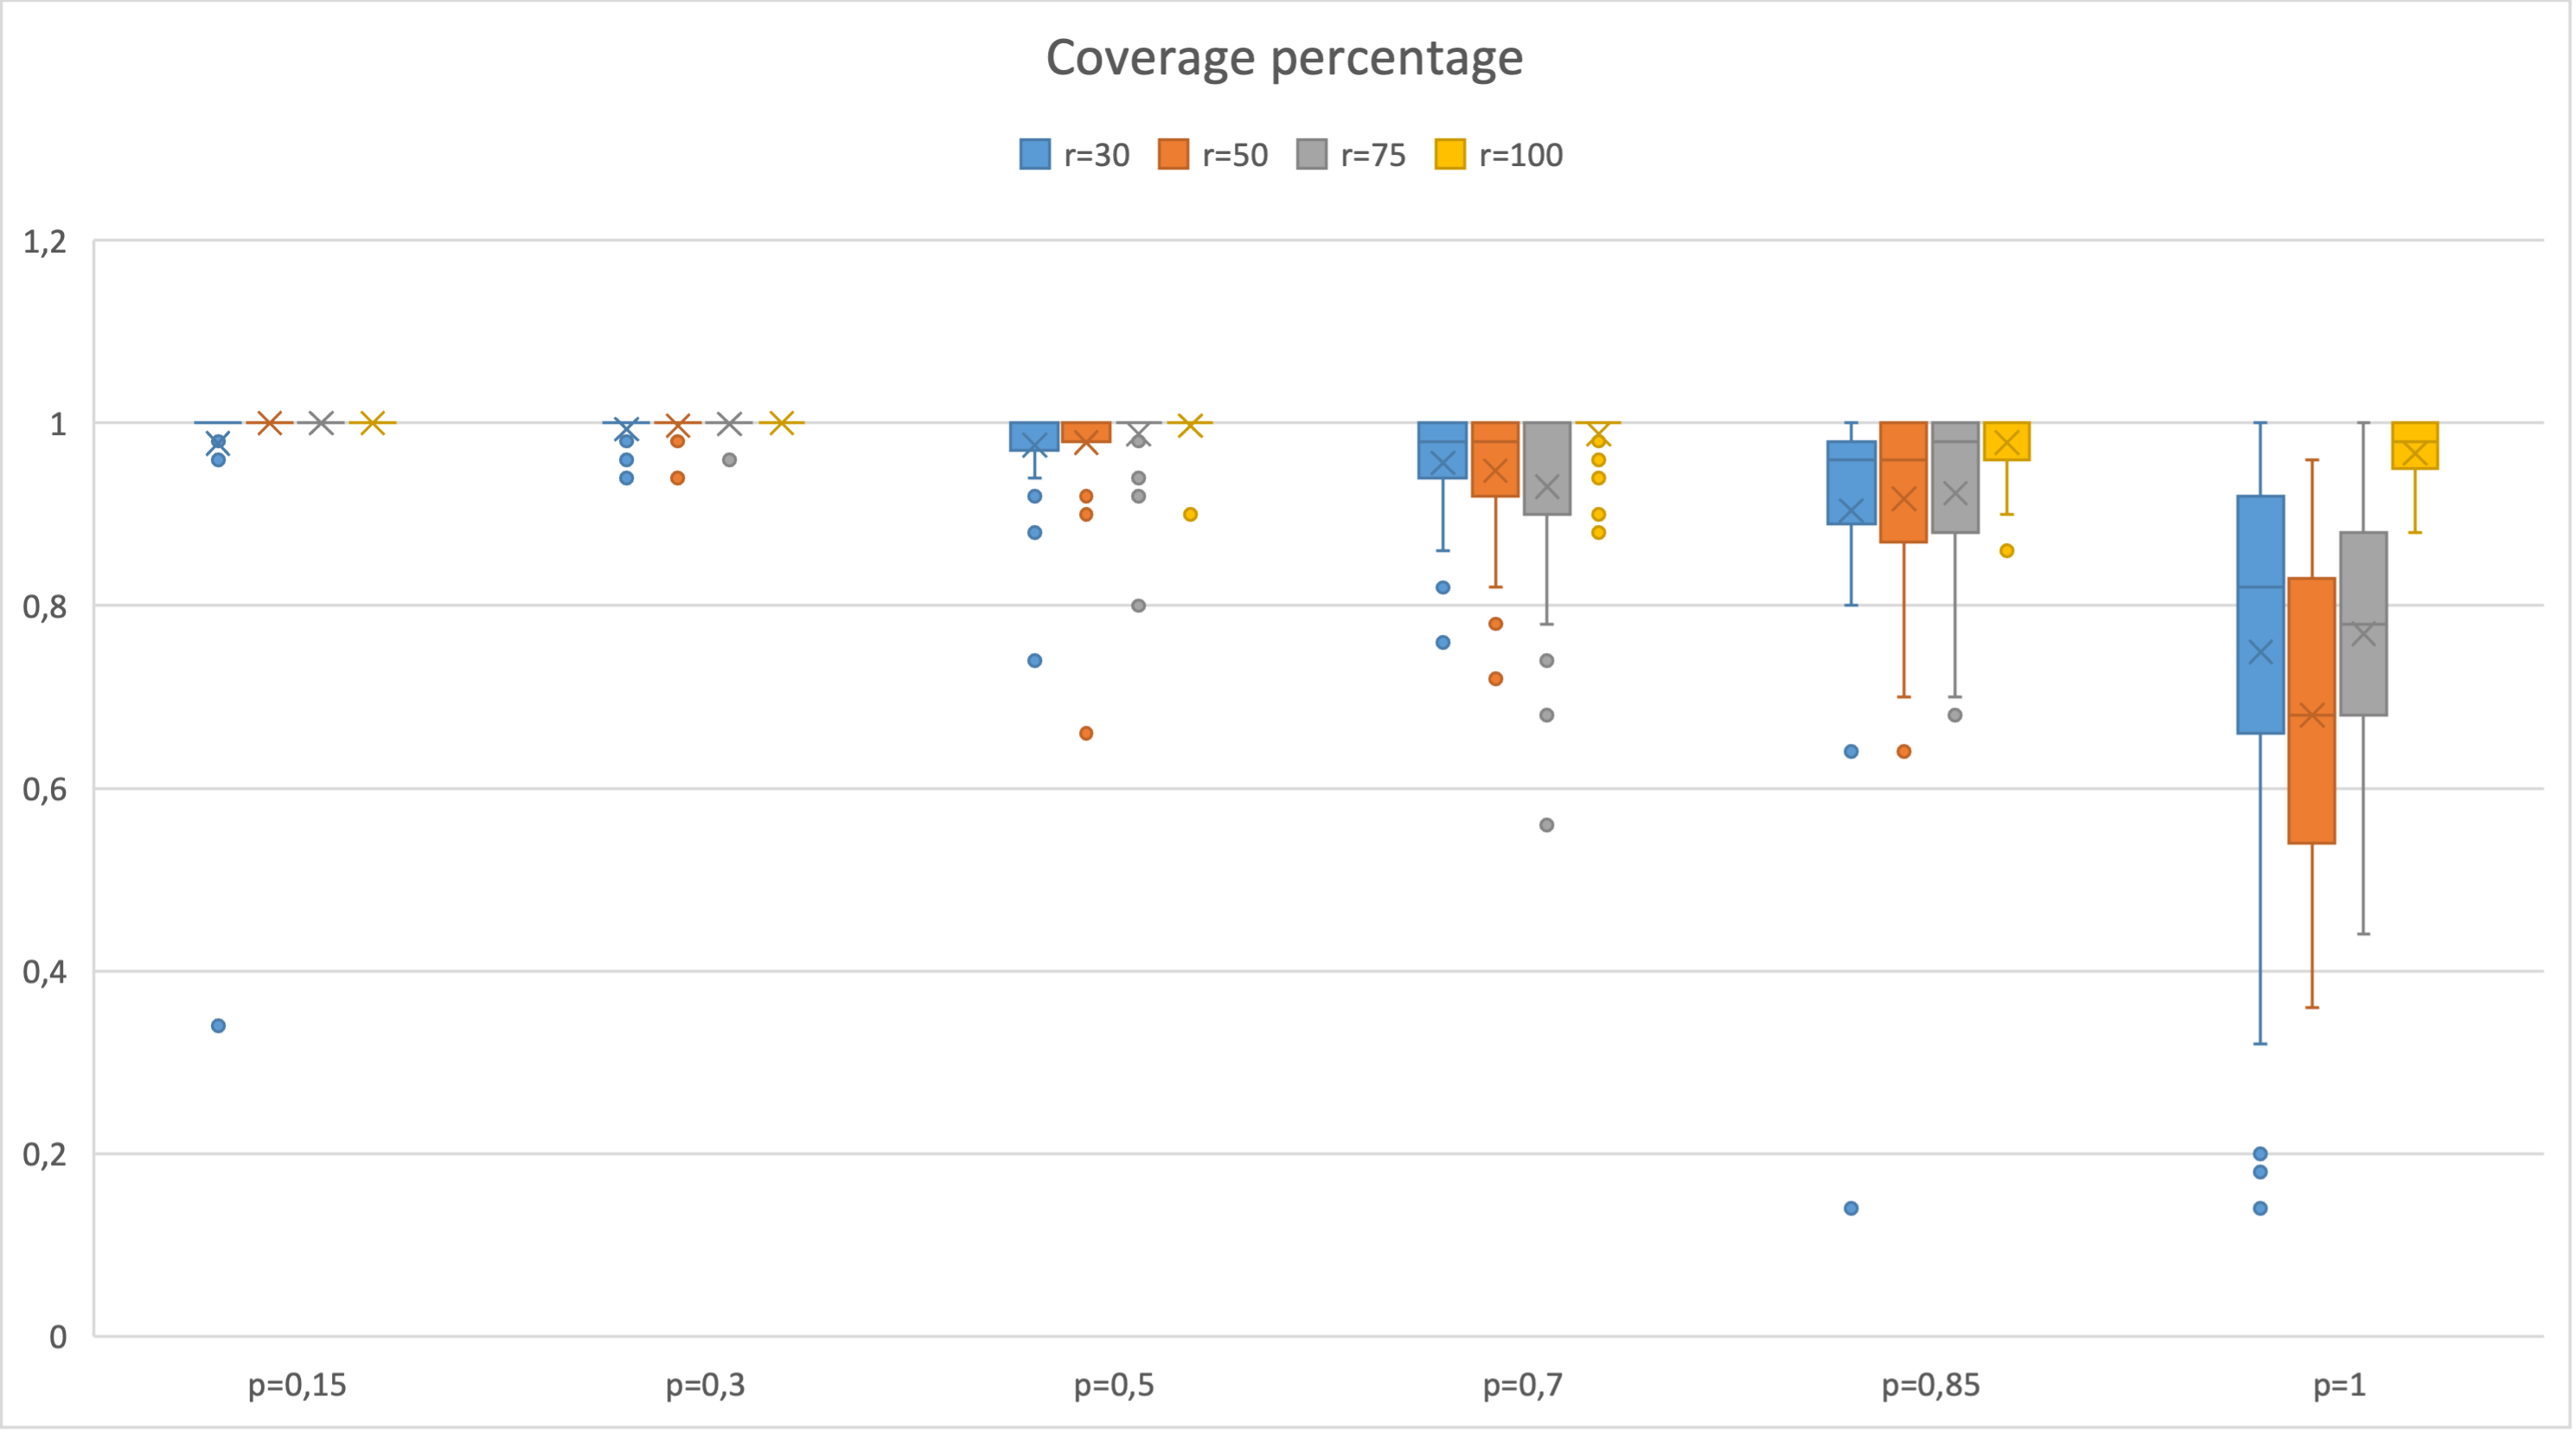
\includegraphics[width=\linewidth]{./images/Rate50Boxplot.png}
  \caption{50 Nodes}\label{fig:awesome_image1}
\endminipage\hfill
\minipage{0.50\linewidth}
  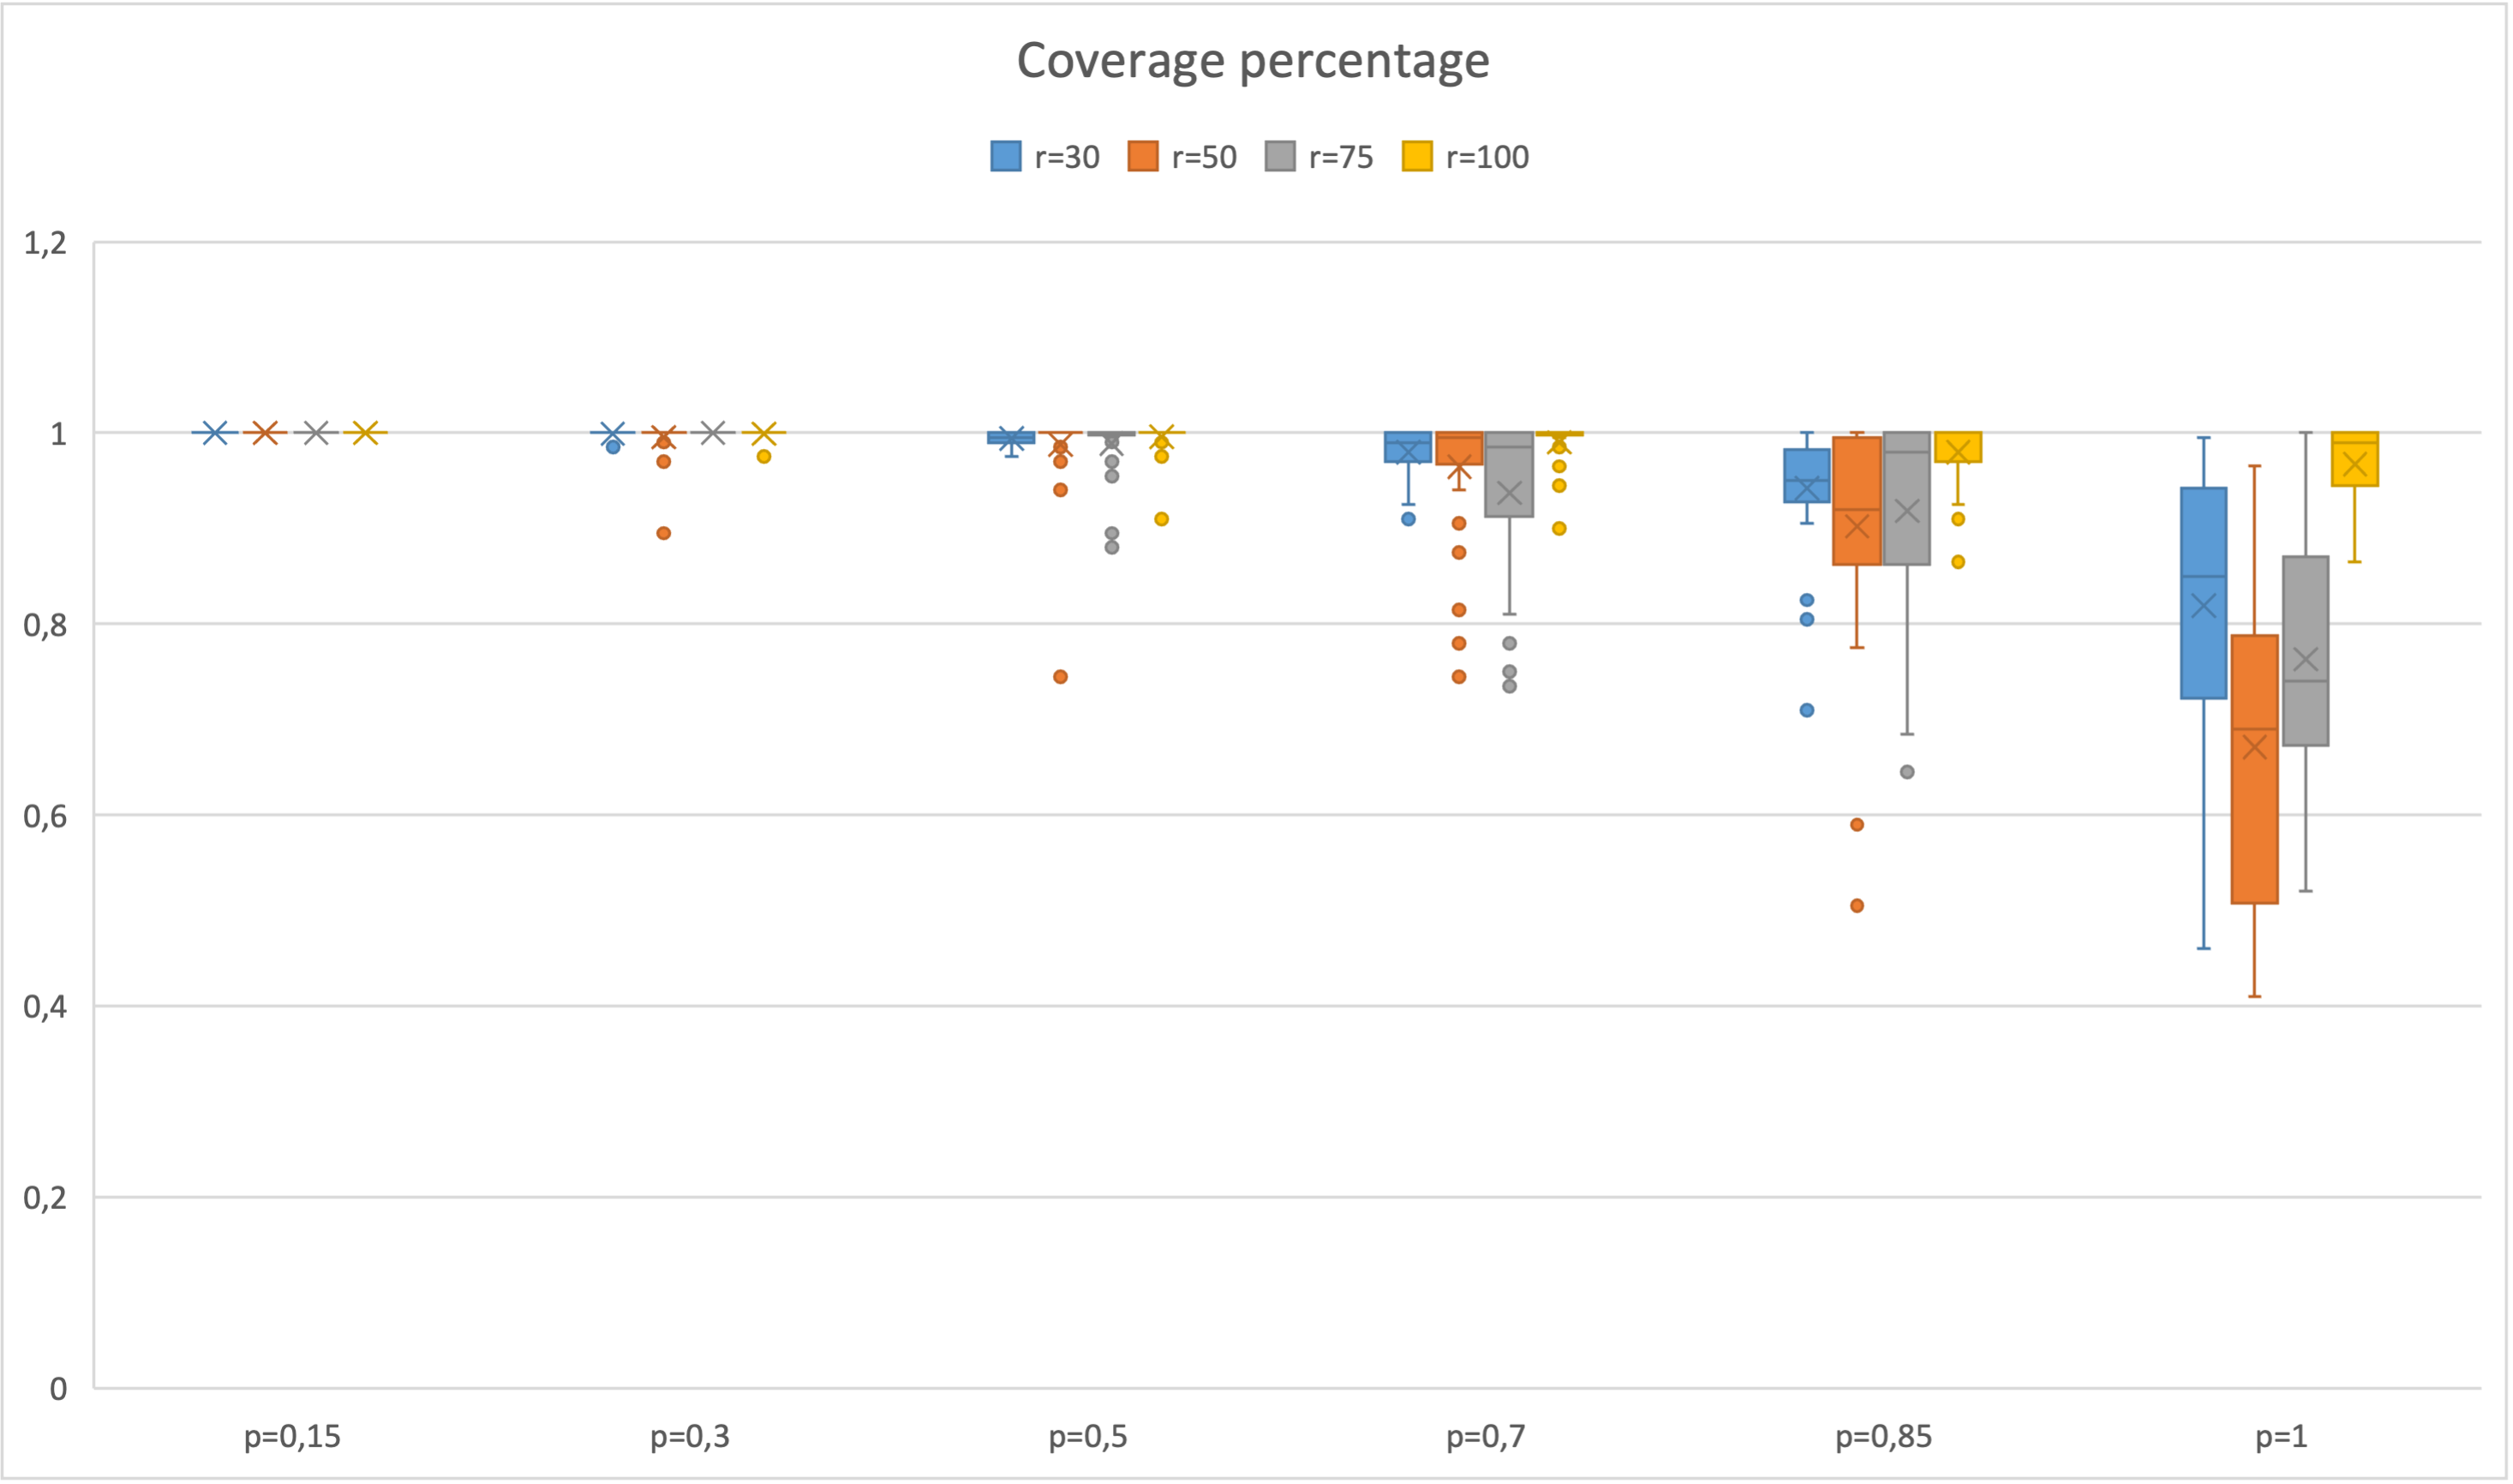
\includegraphics[width=\linewidth]{./images/Rate200Boxplot.png}
  \caption{200 Nodes}\label{fig:awesome_image2}
\endminipage
\end{figure}

\begin{figure}[H]
\minipage{0.50\linewidth}
  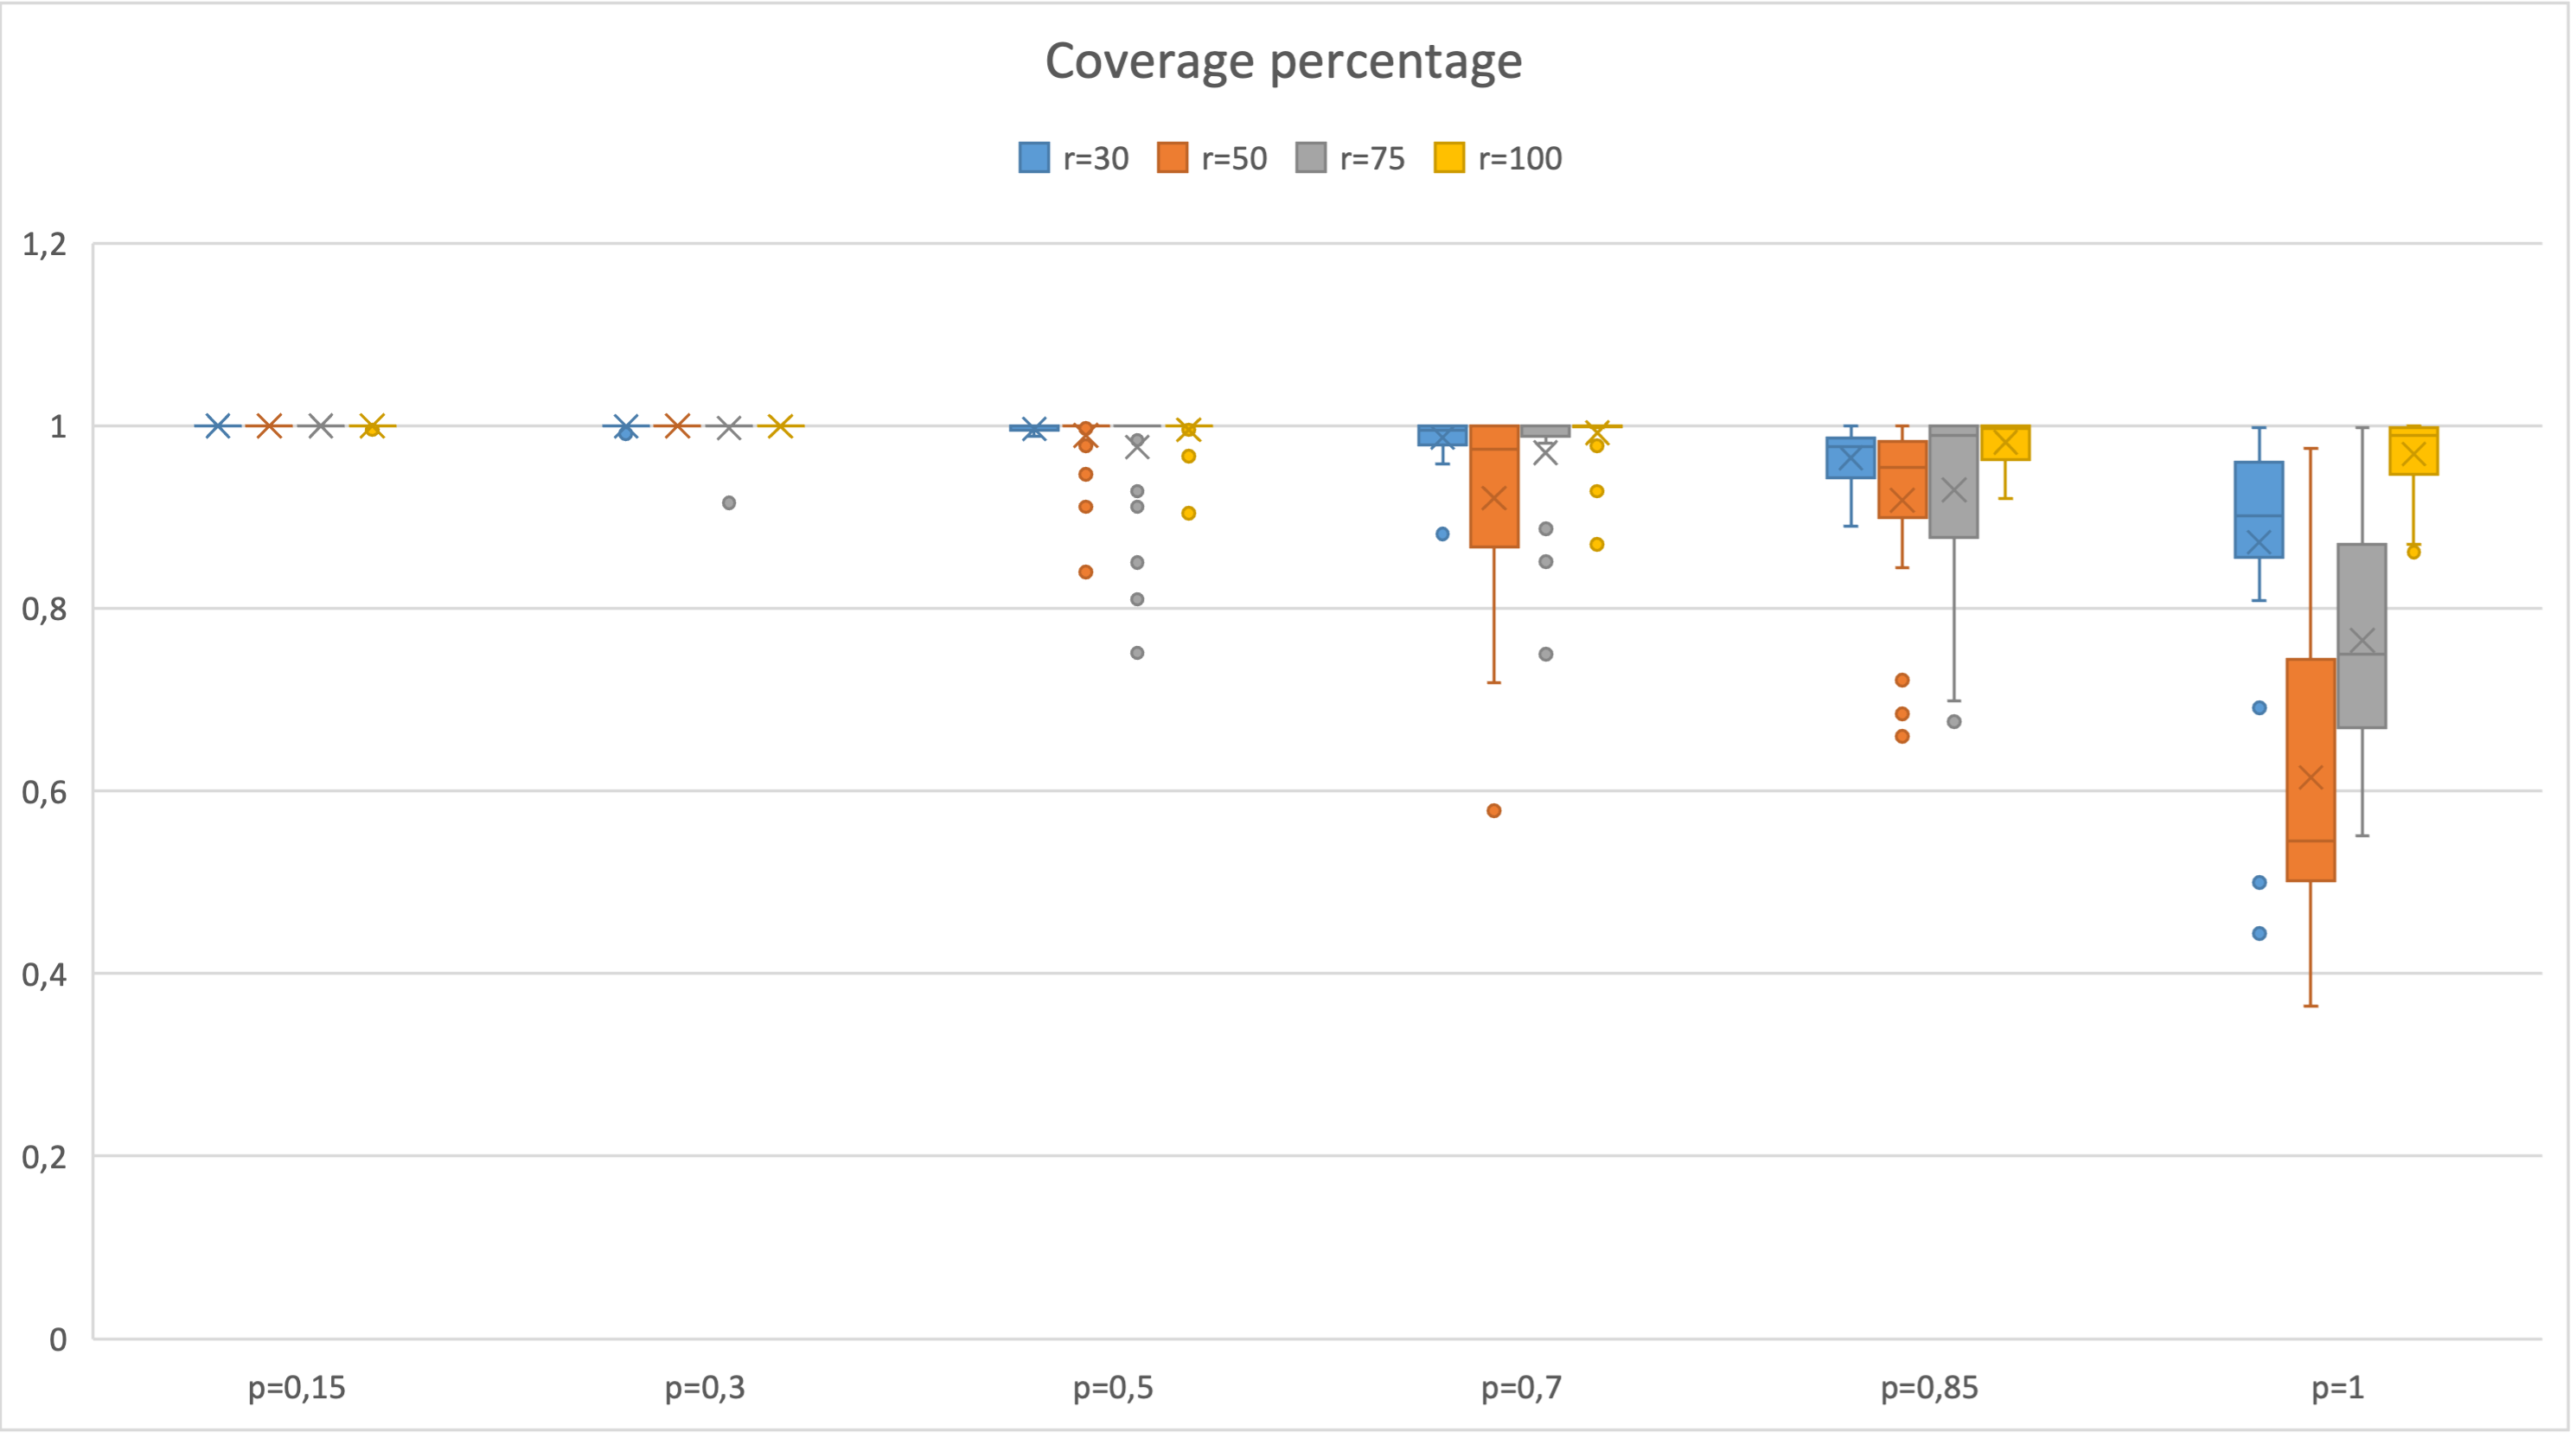
\includegraphics[width=\linewidth]{./images/Rate700Boxplot.png}
  \caption{700 Nodes}\label{fig:awesome_image1}
\endminipage\hfill
\minipage{0.50\linewidth}
  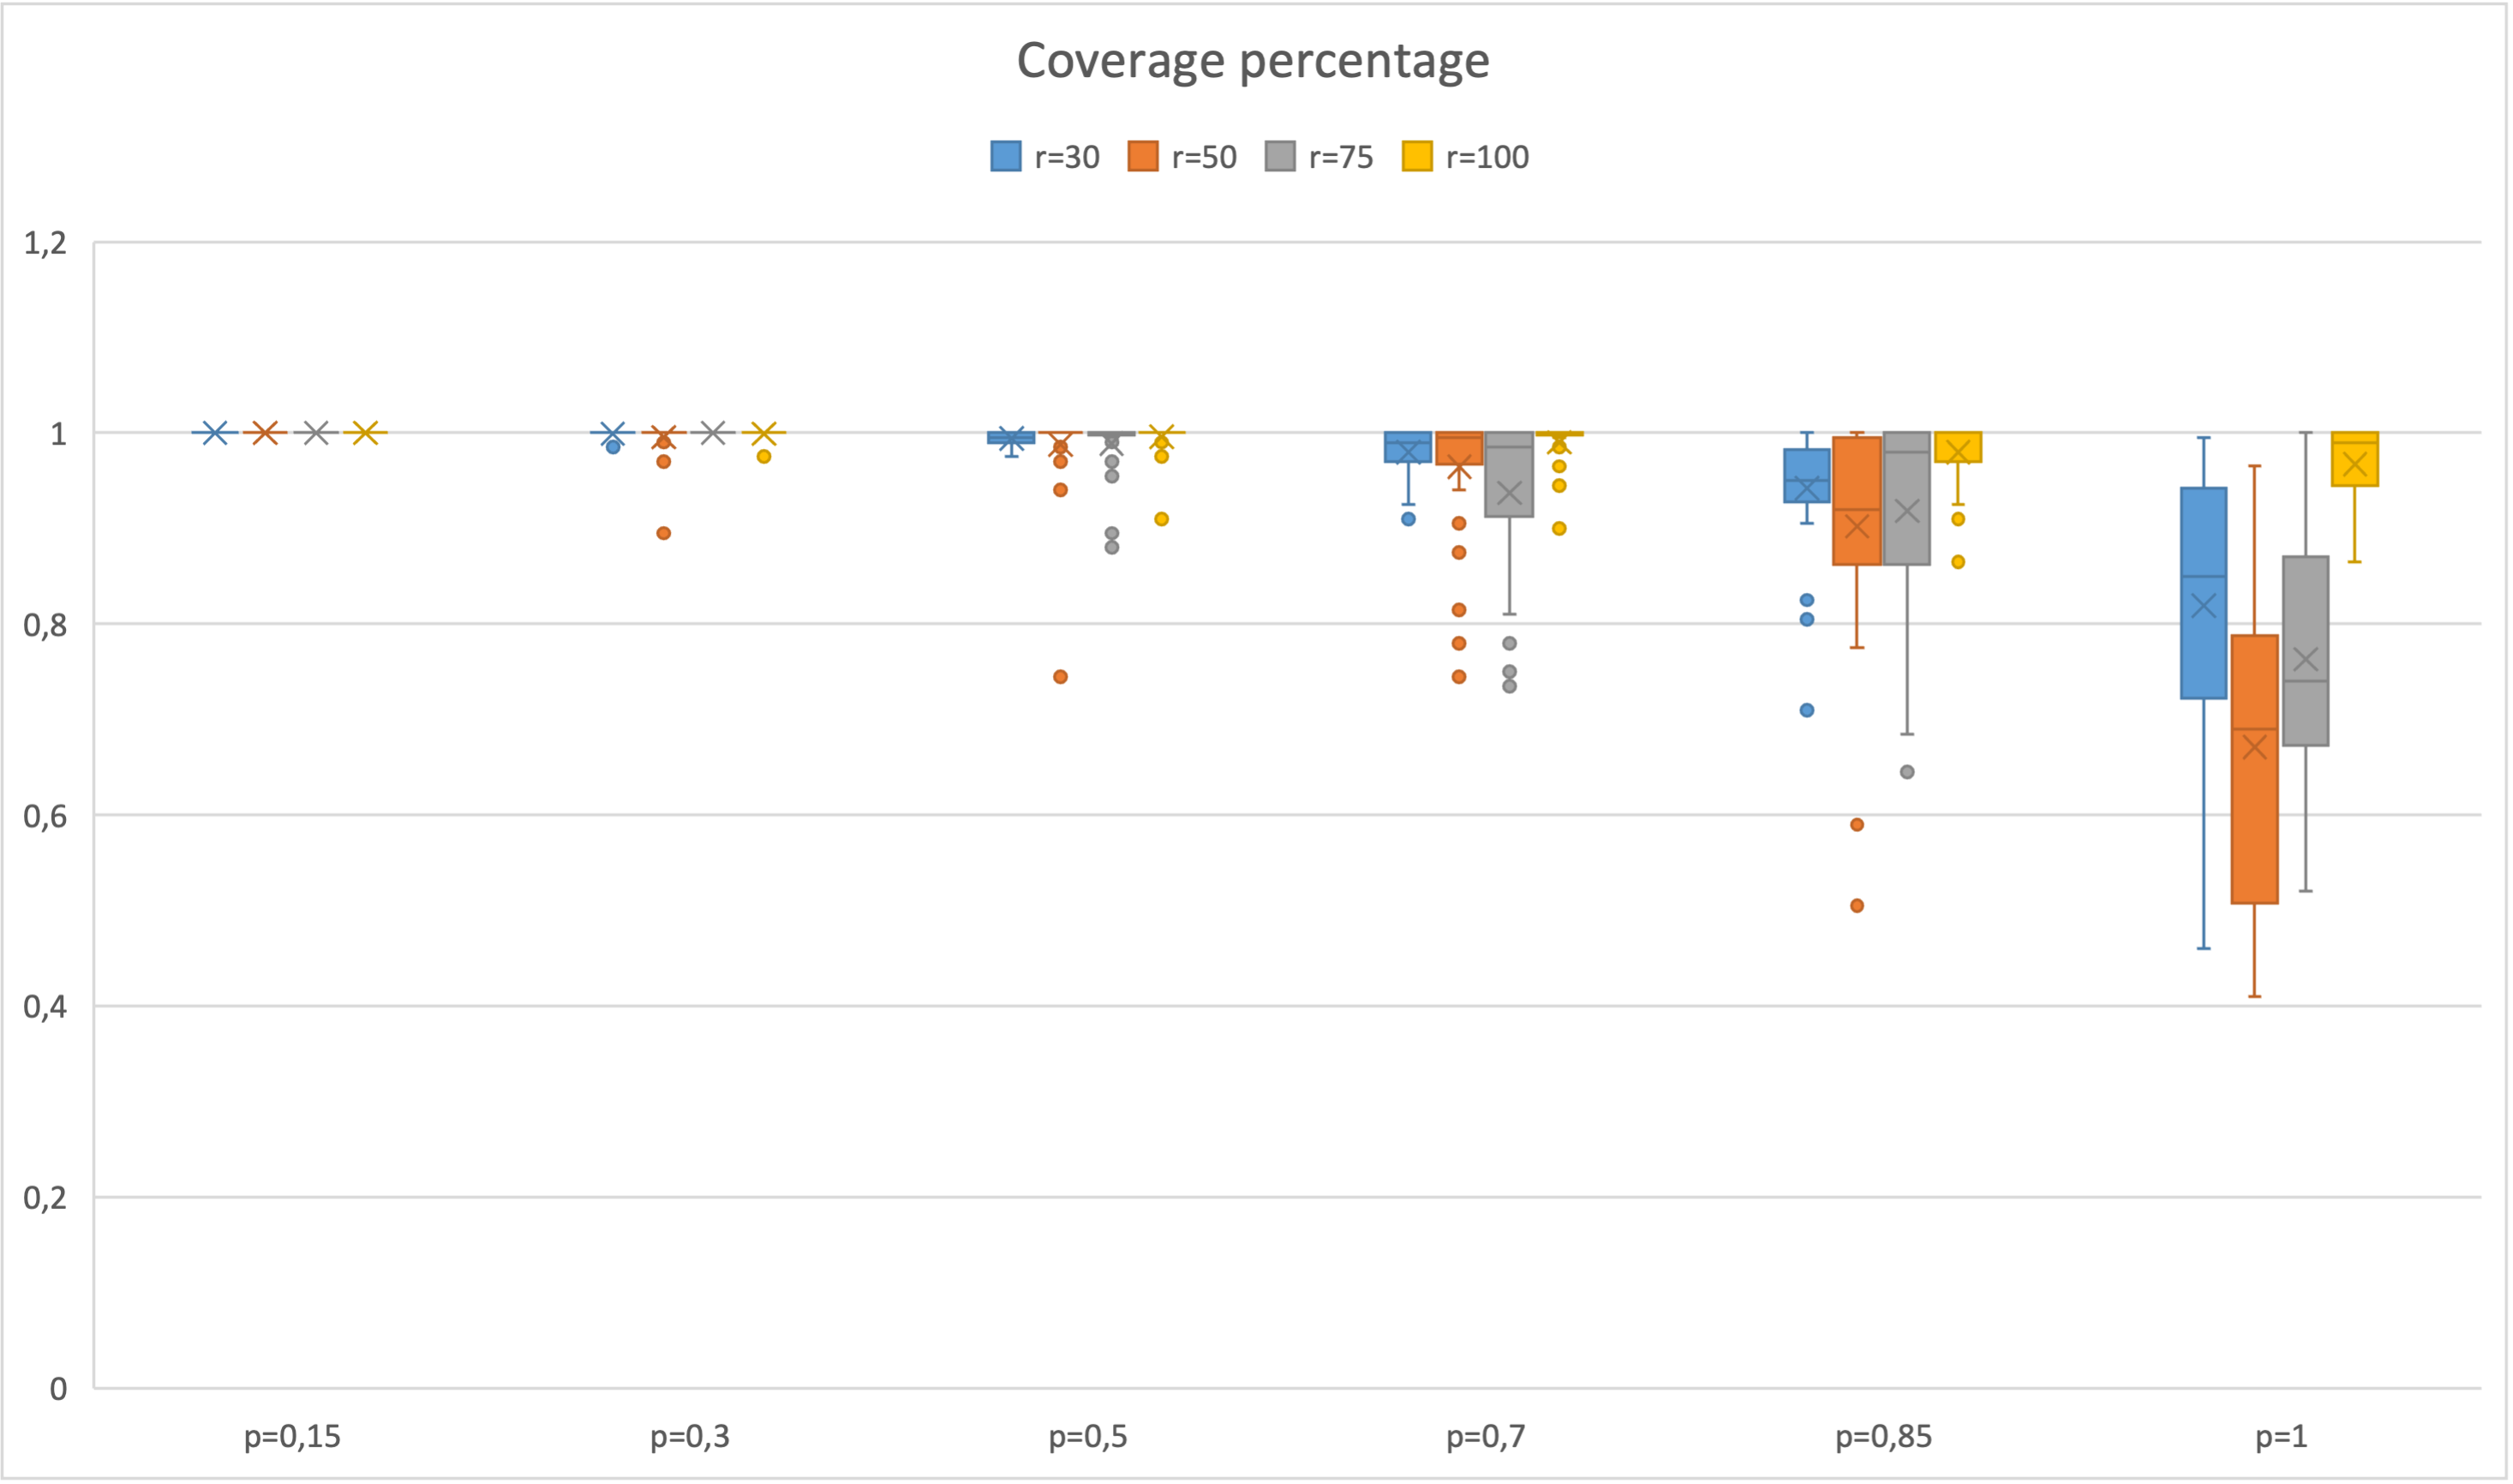
\includegraphics[width=\linewidth]{./images/Rate200Boxplot.png}
  \caption{200 Nodes}\label{fig:awesome_image2}
\endminipage
\end{figure}



\subsection{Coverage time}
\begin{figure}[H]
\minipage{0.50\linewidth}
  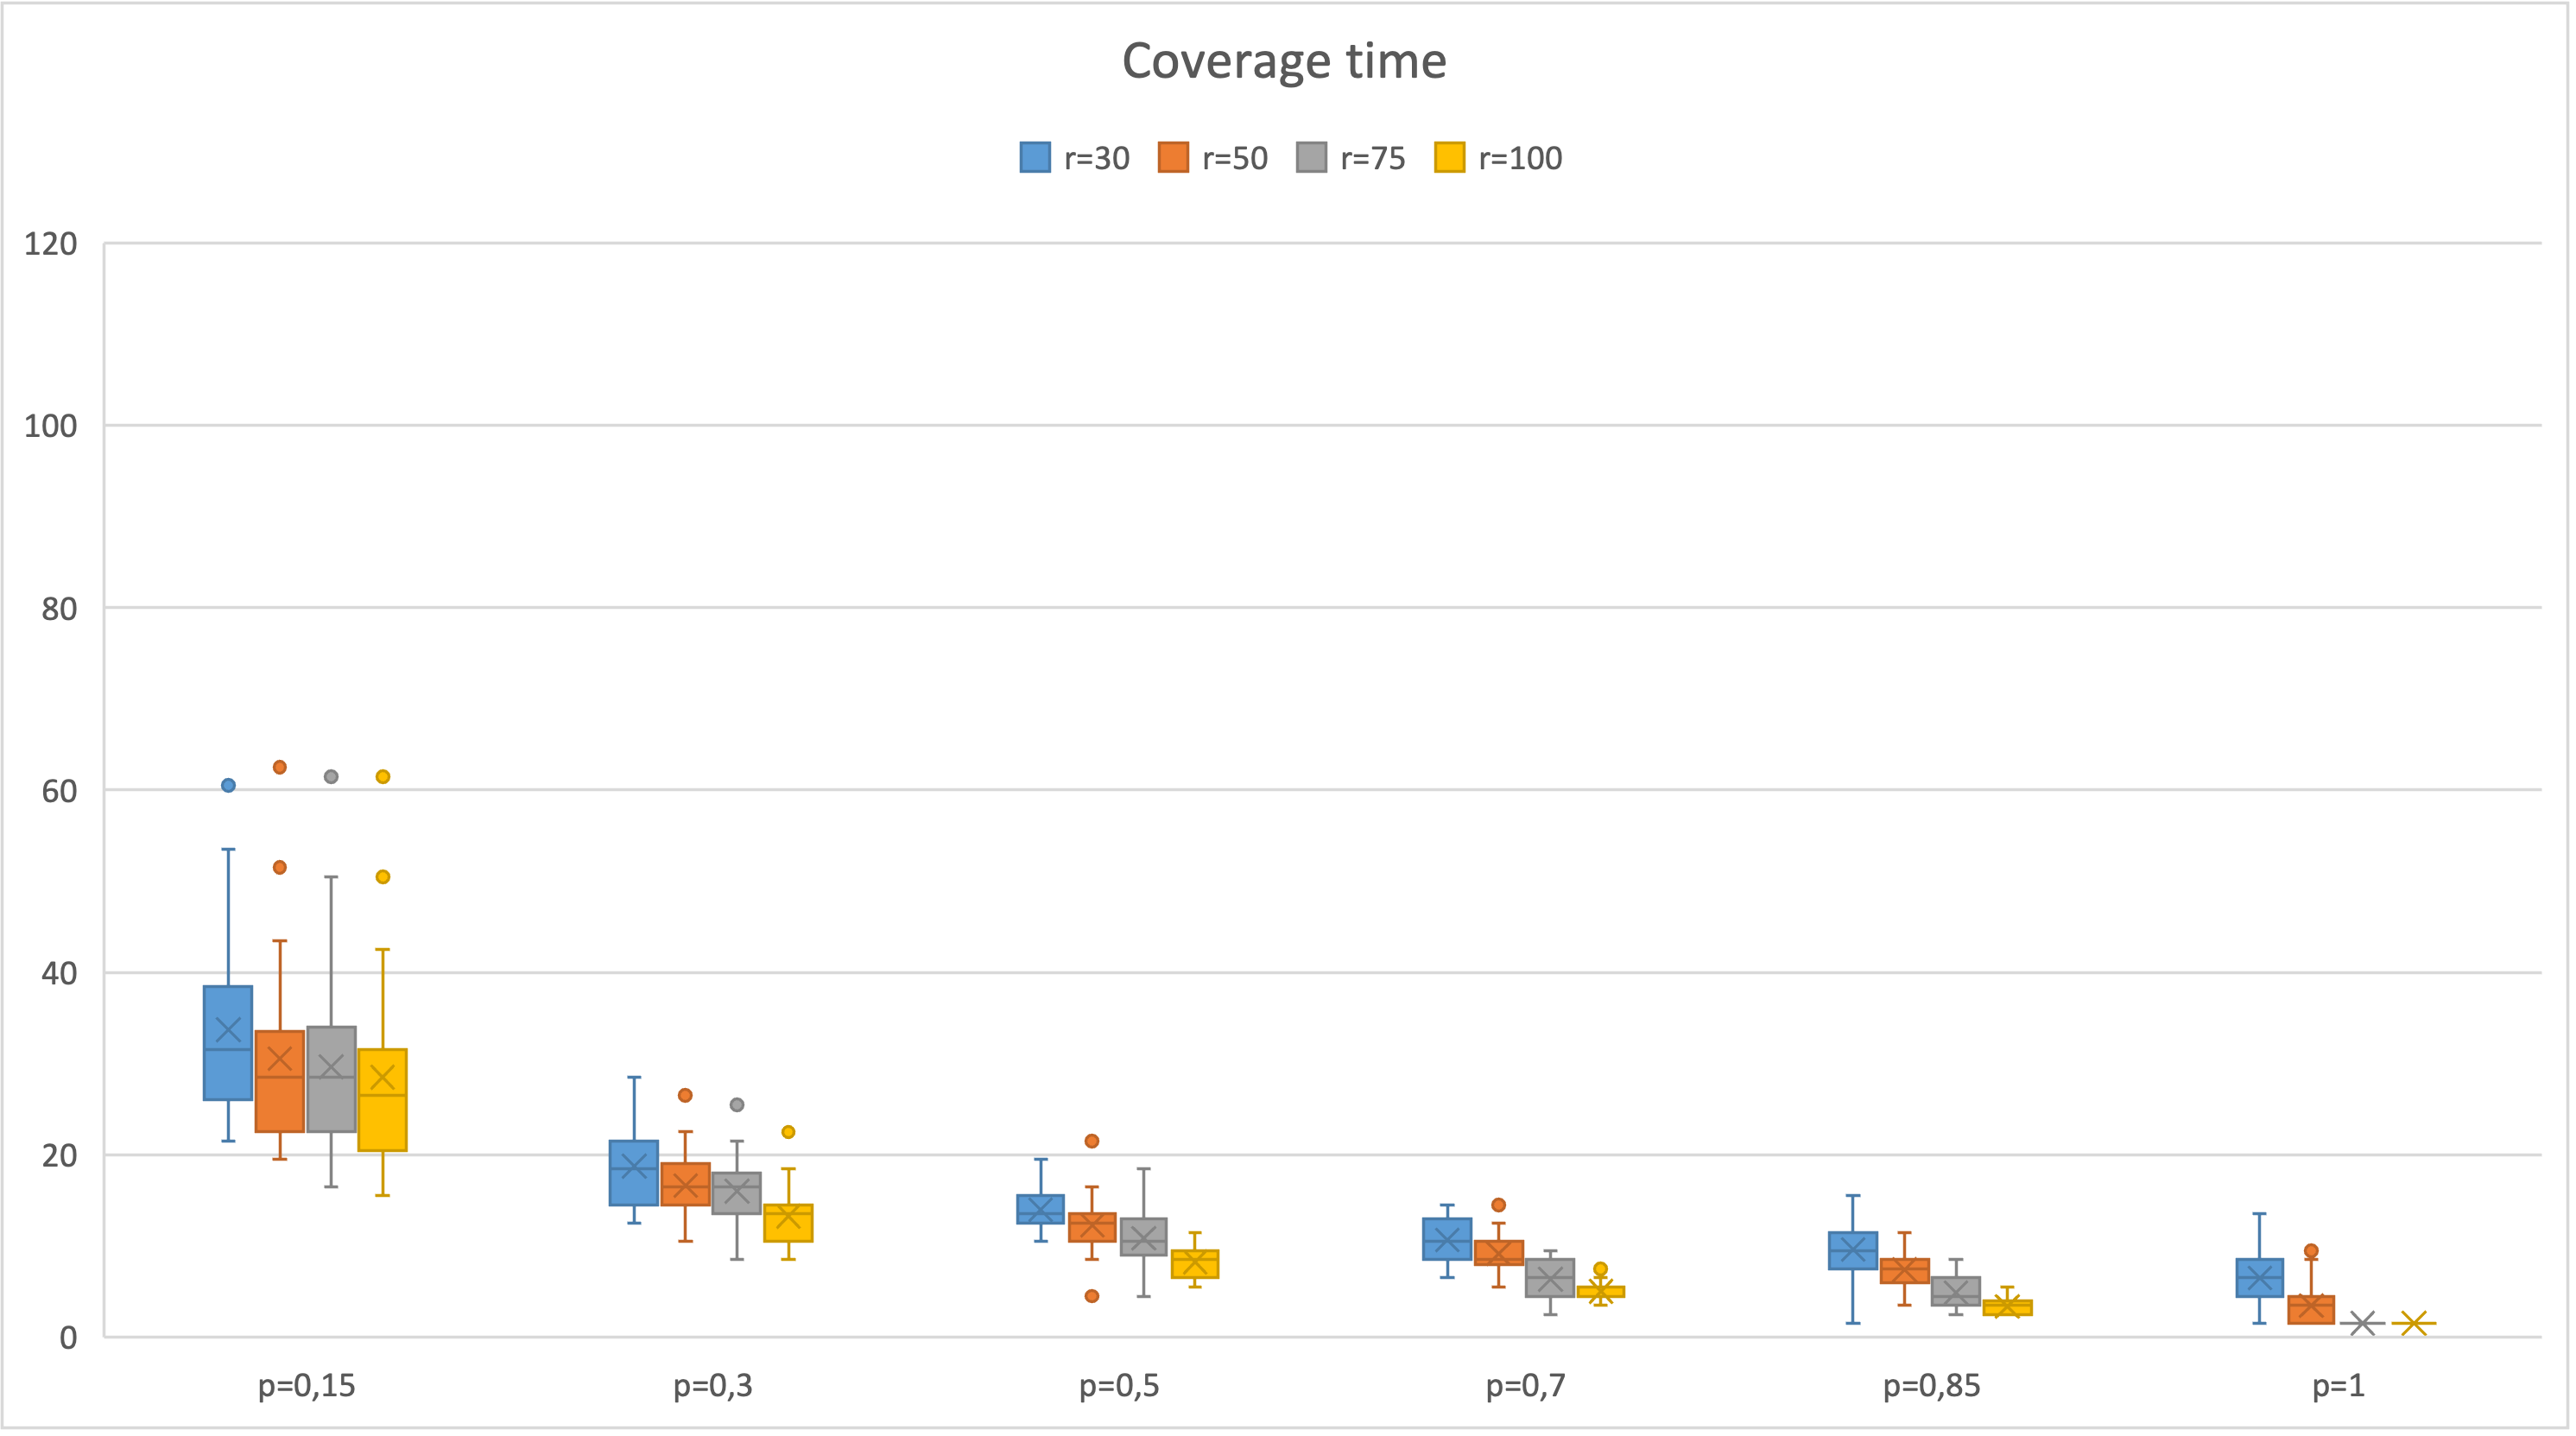
\includegraphics[width=\linewidth]{./images/Time50Boxplot.png}
  \caption{50 Nodes}\label{fig:awesome_image1}
\endminipage\hfill
\minipage{0.50\linewidth}
  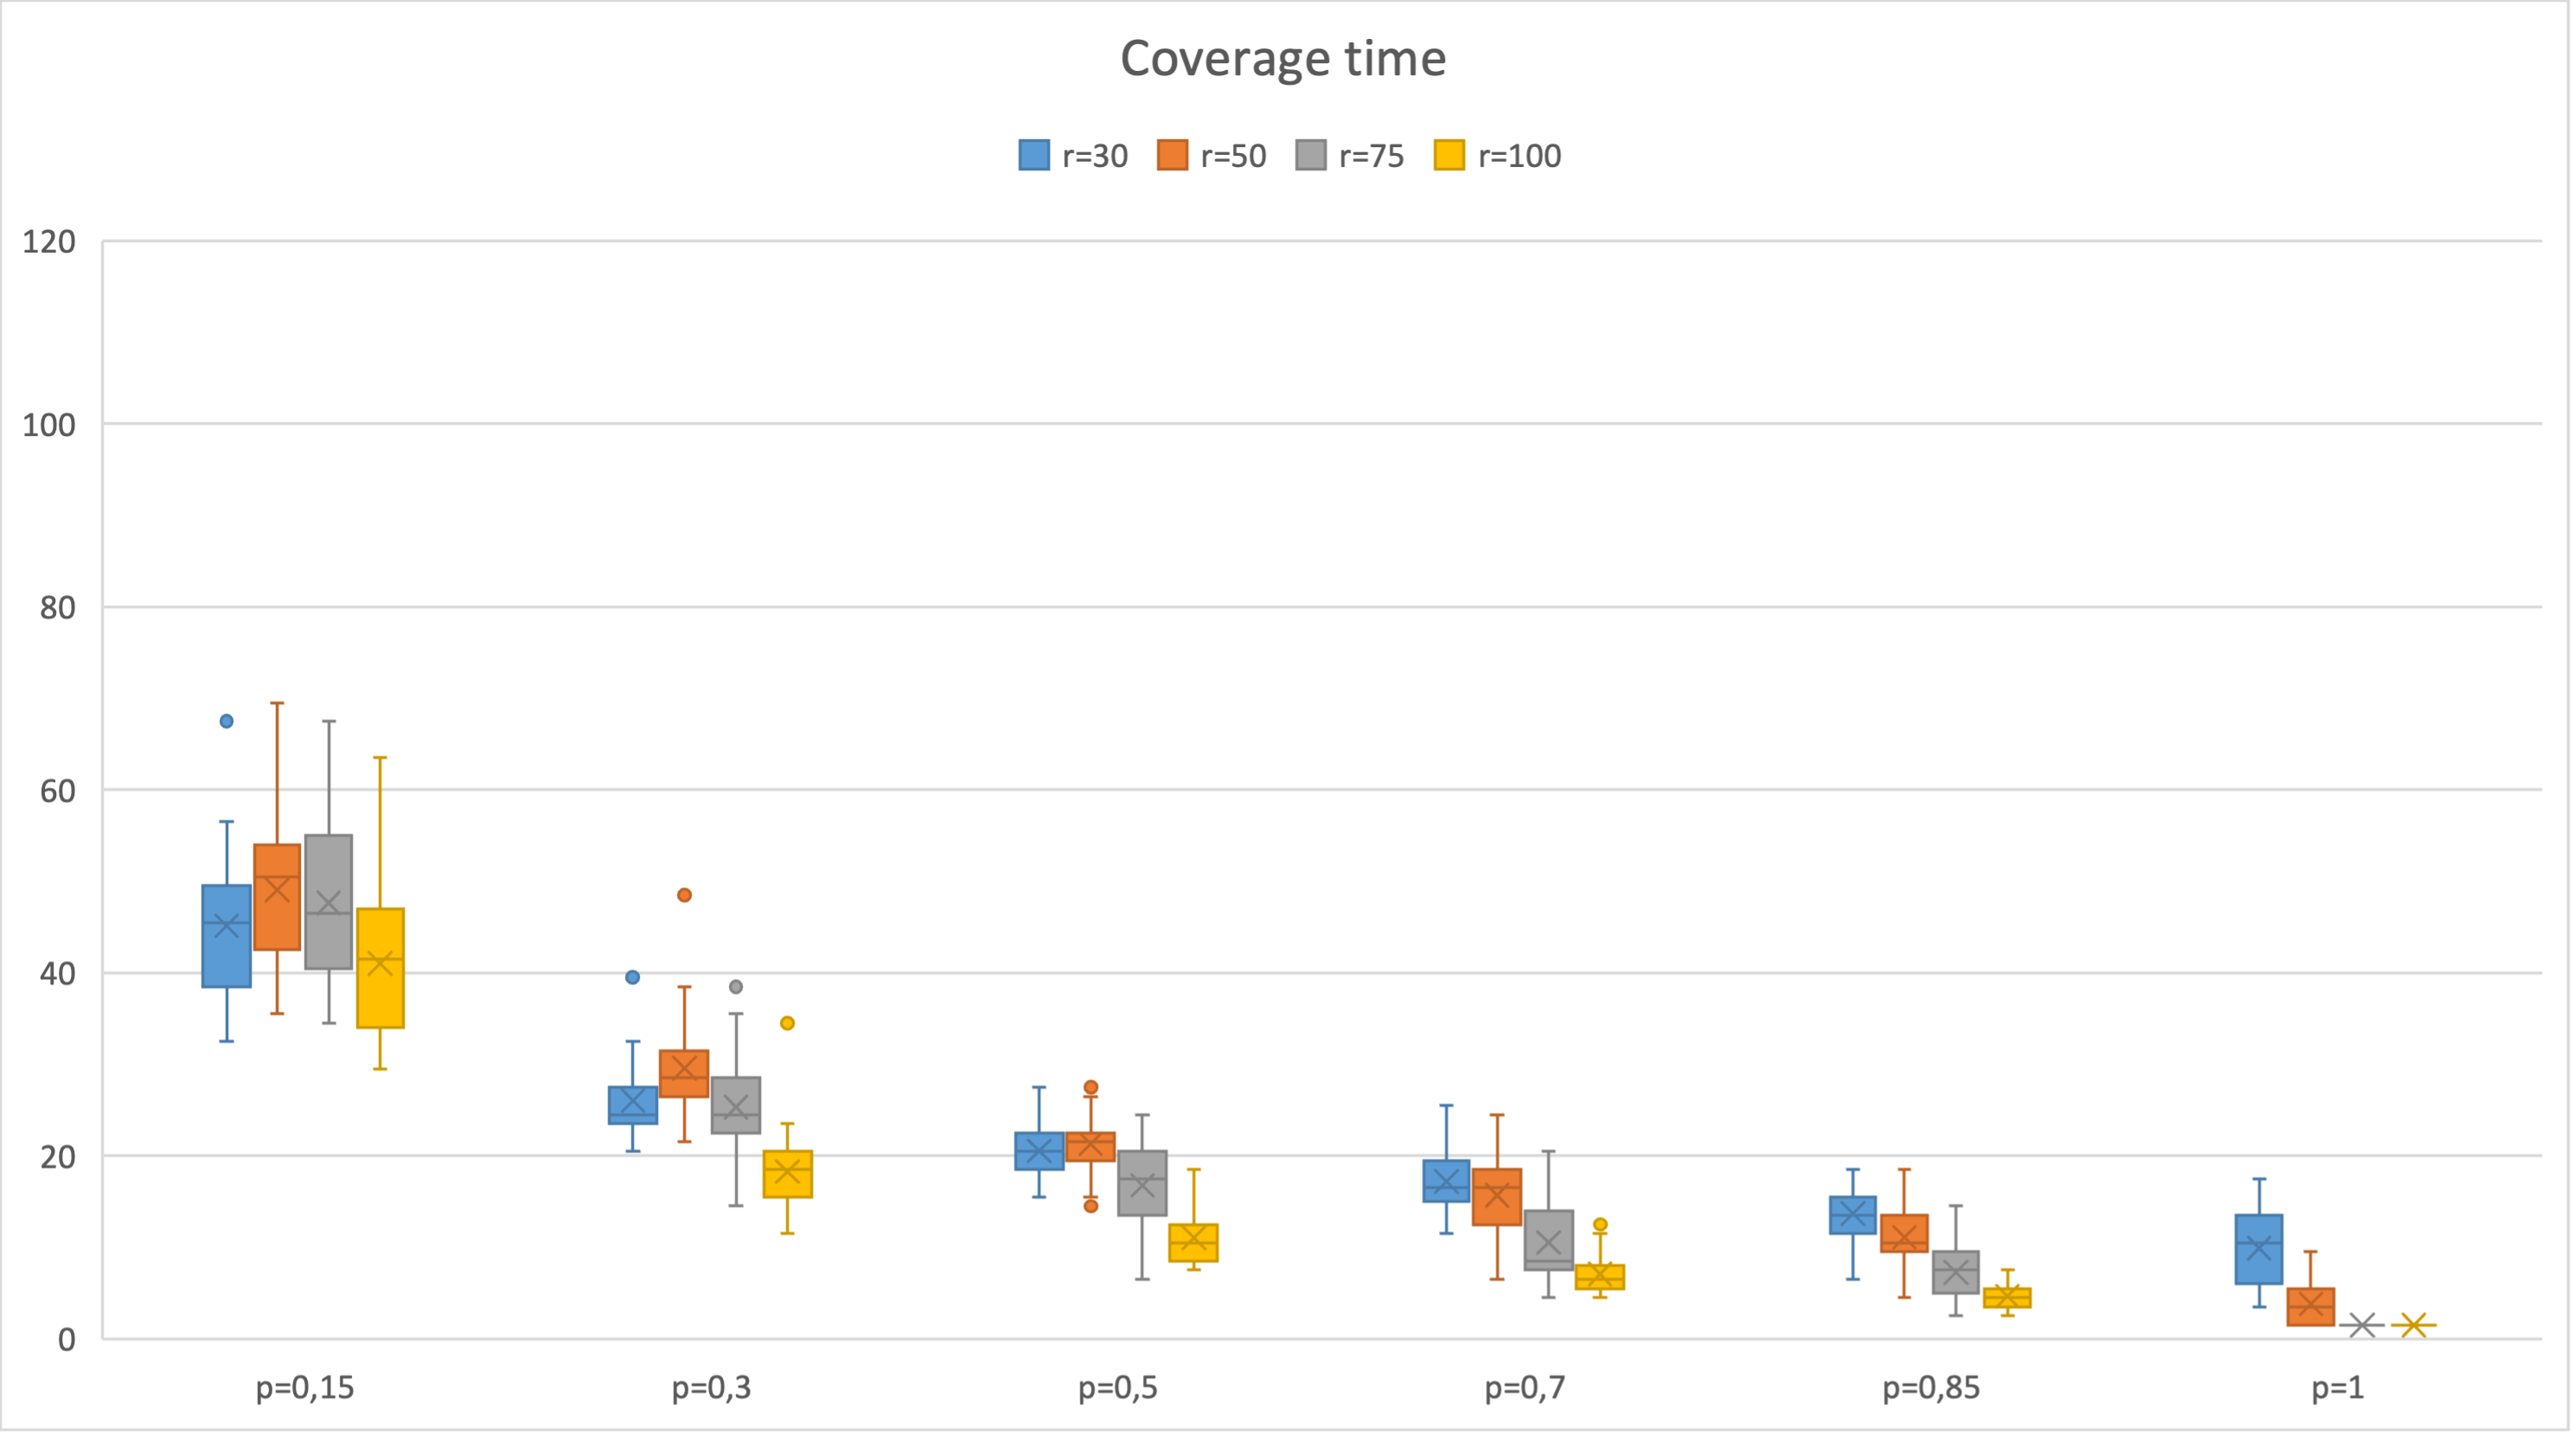
\includegraphics[width=\linewidth]{./images/Time200BoxplotScaled.png}
  \caption{200 Nodes}\label{fig:awesome_image2}
\endminipage
\end{figure}

\begin{figure}[H]
\minipage{0.50\linewidth}
  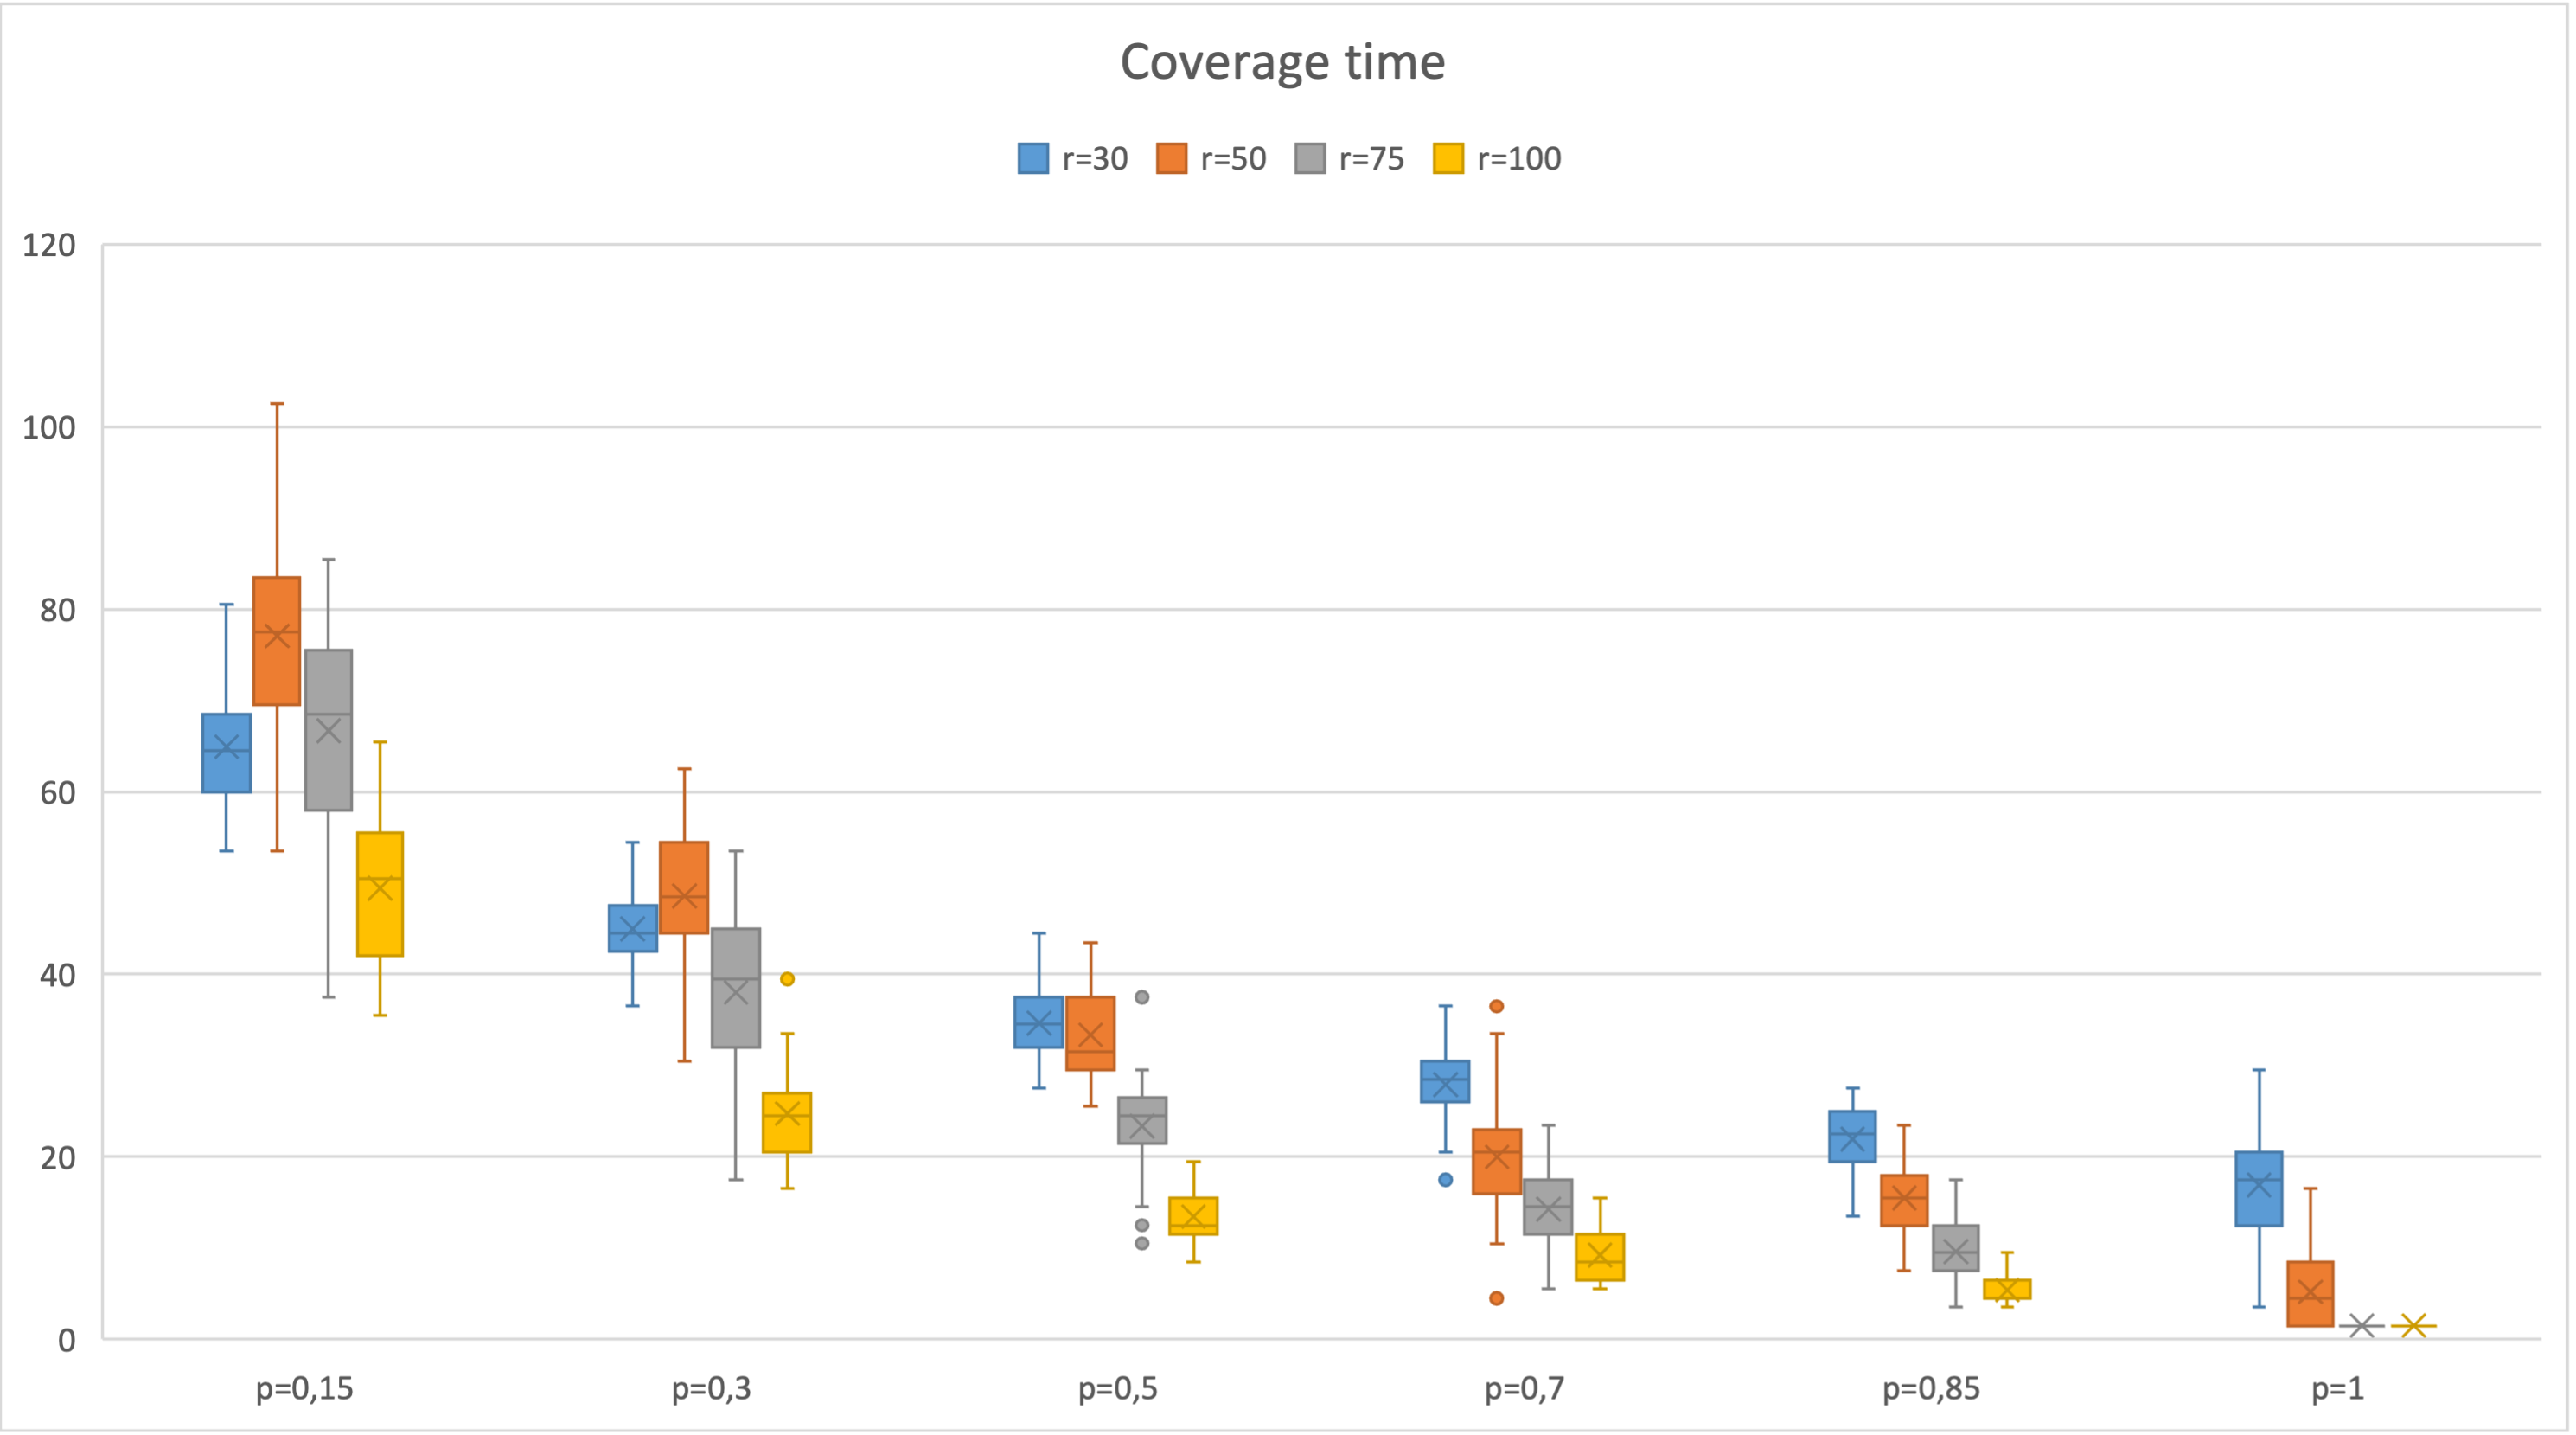
\includegraphics[width=\linewidth]{./images/Time700Boxplot.png}
  \caption{700 Nodes}\label{fig:awesome_image1}
\endminipage\hfill
\minipage{0.50\linewidth}
  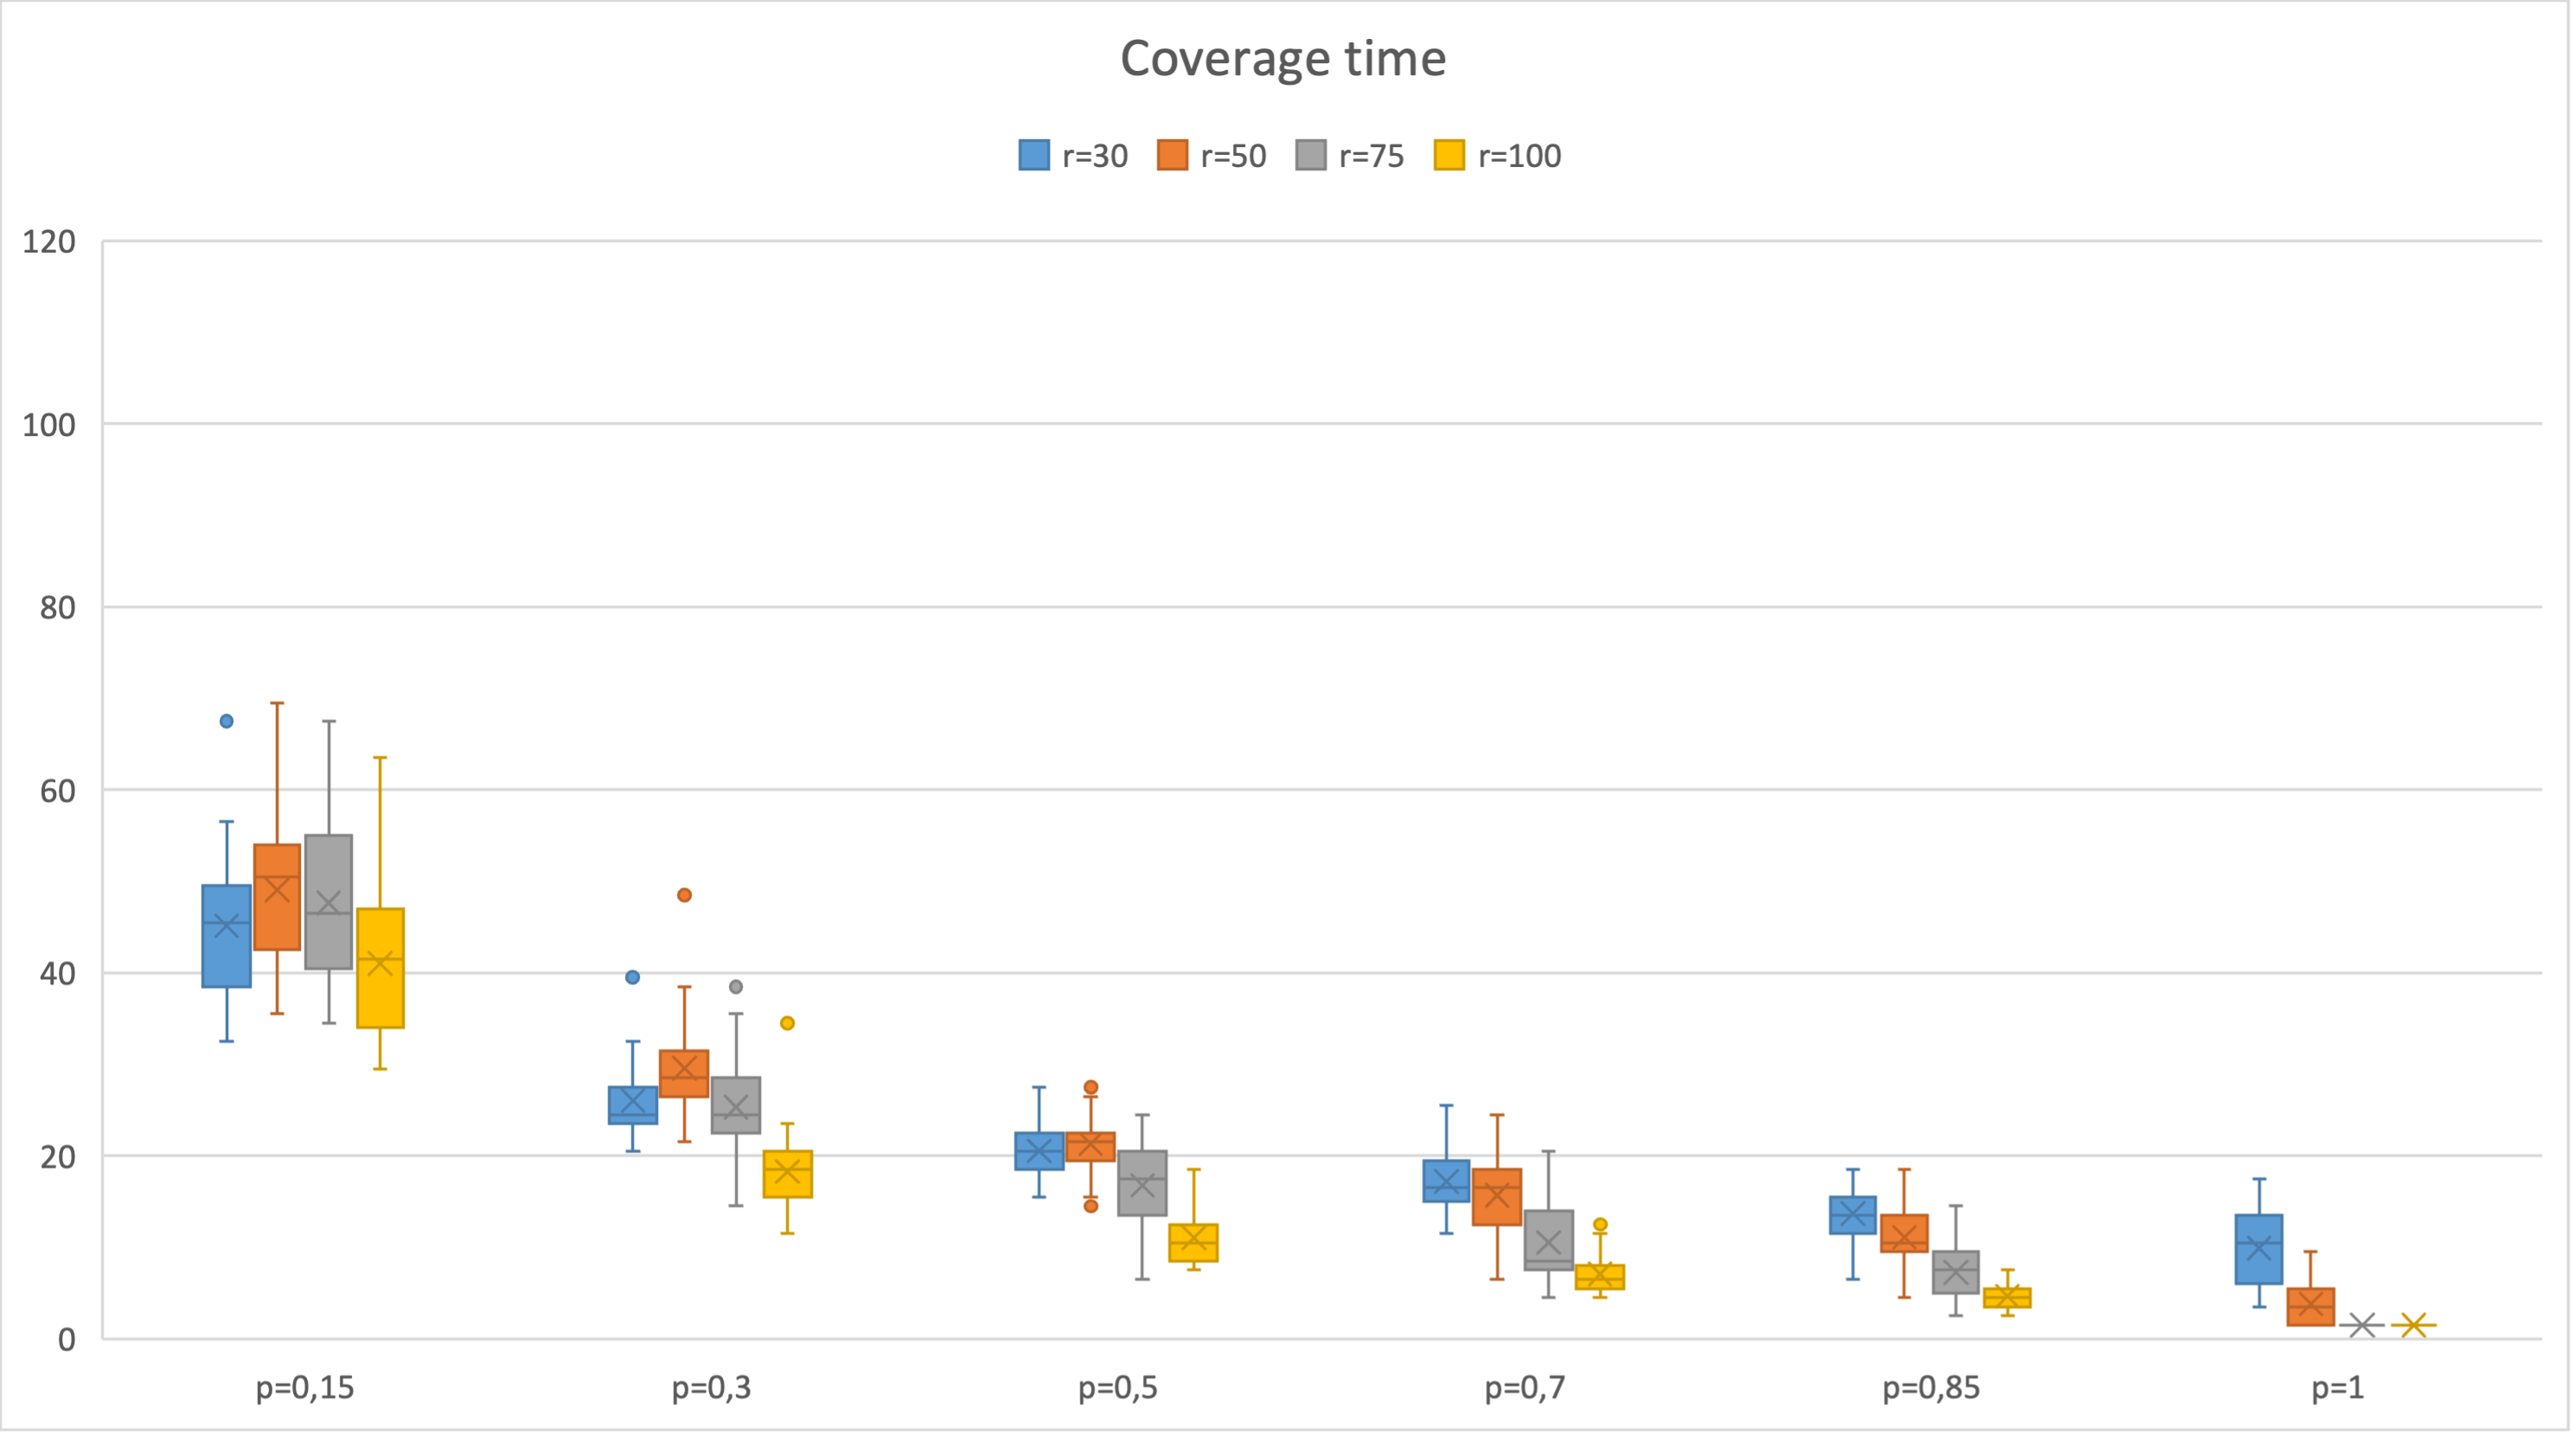
\includegraphics[width=\linewidth]{./images/Time200BoxplotScaled.png}
  \caption{200 Nodes}\label{fig:awesome_image2}
\endminipage
\end{figure}

\subsection{Collision rate}
\begin{figure}[H]
\minipage{0.50\linewidth}
  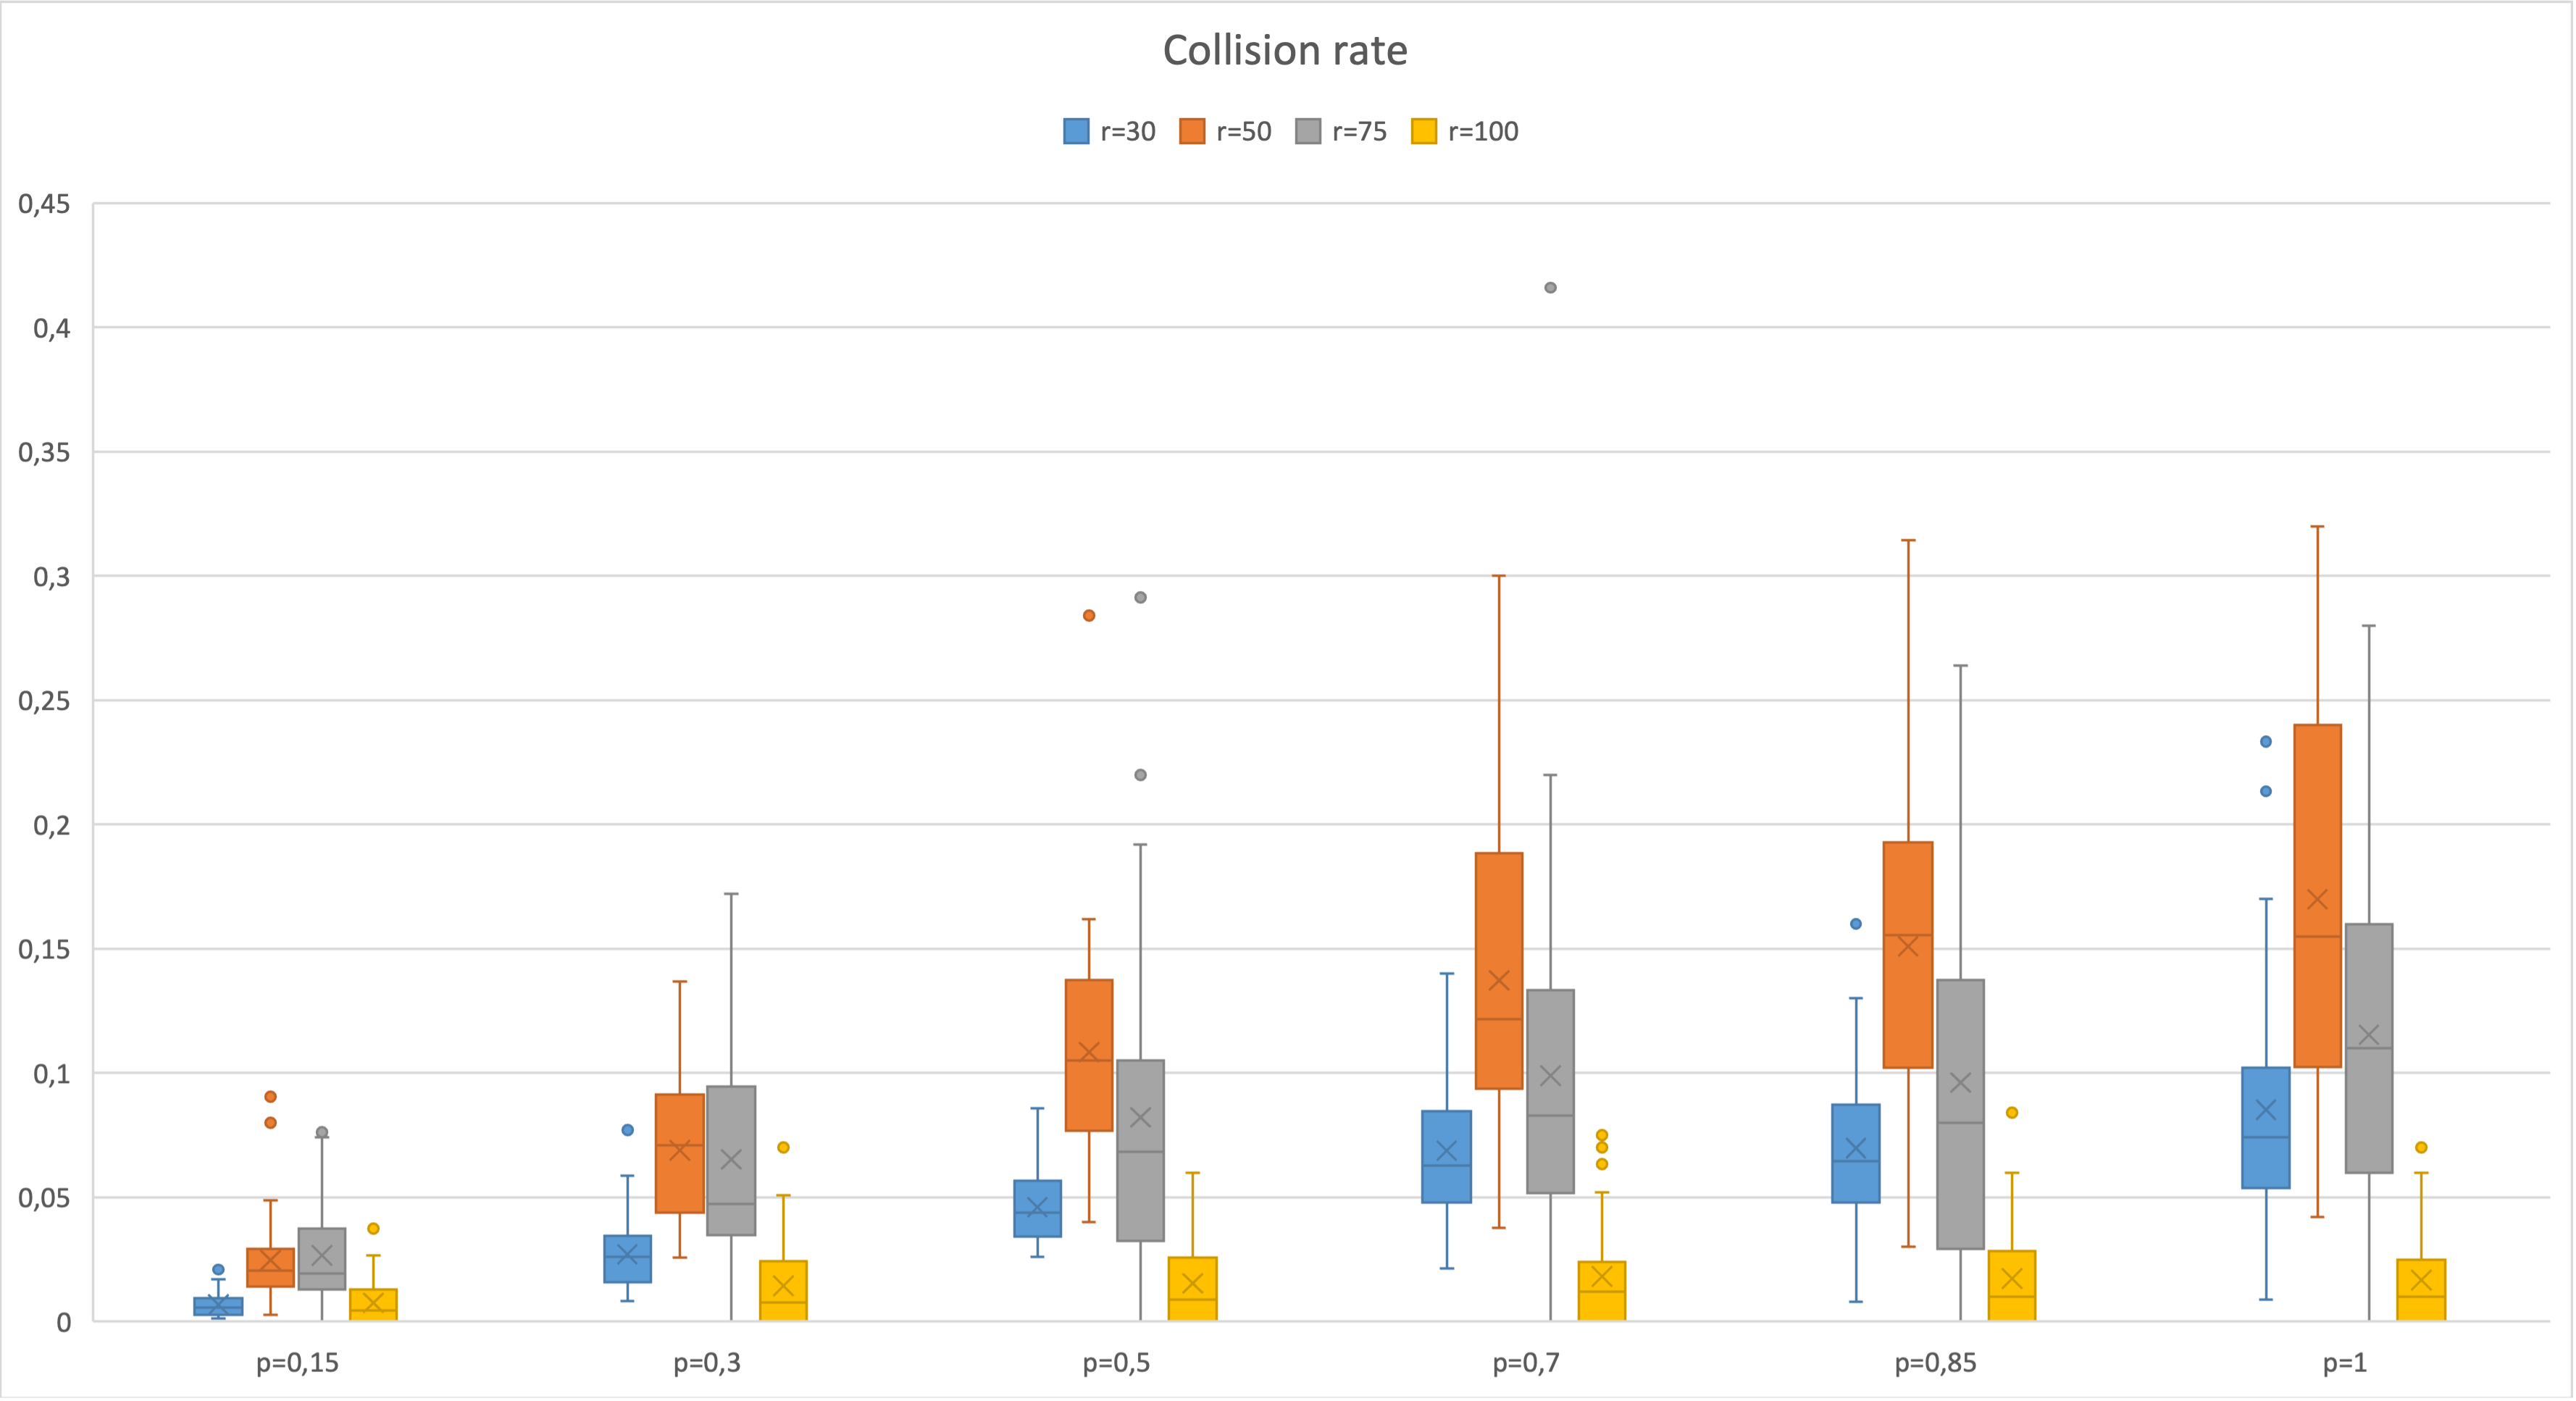
\includegraphics[width=\linewidth]{./images/Collision50Boxplot.png}
  \caption{50 Nodes}\label{fig:awesome_image1}
\endminipage\hfill
\minipage{0.50\linewidth}
  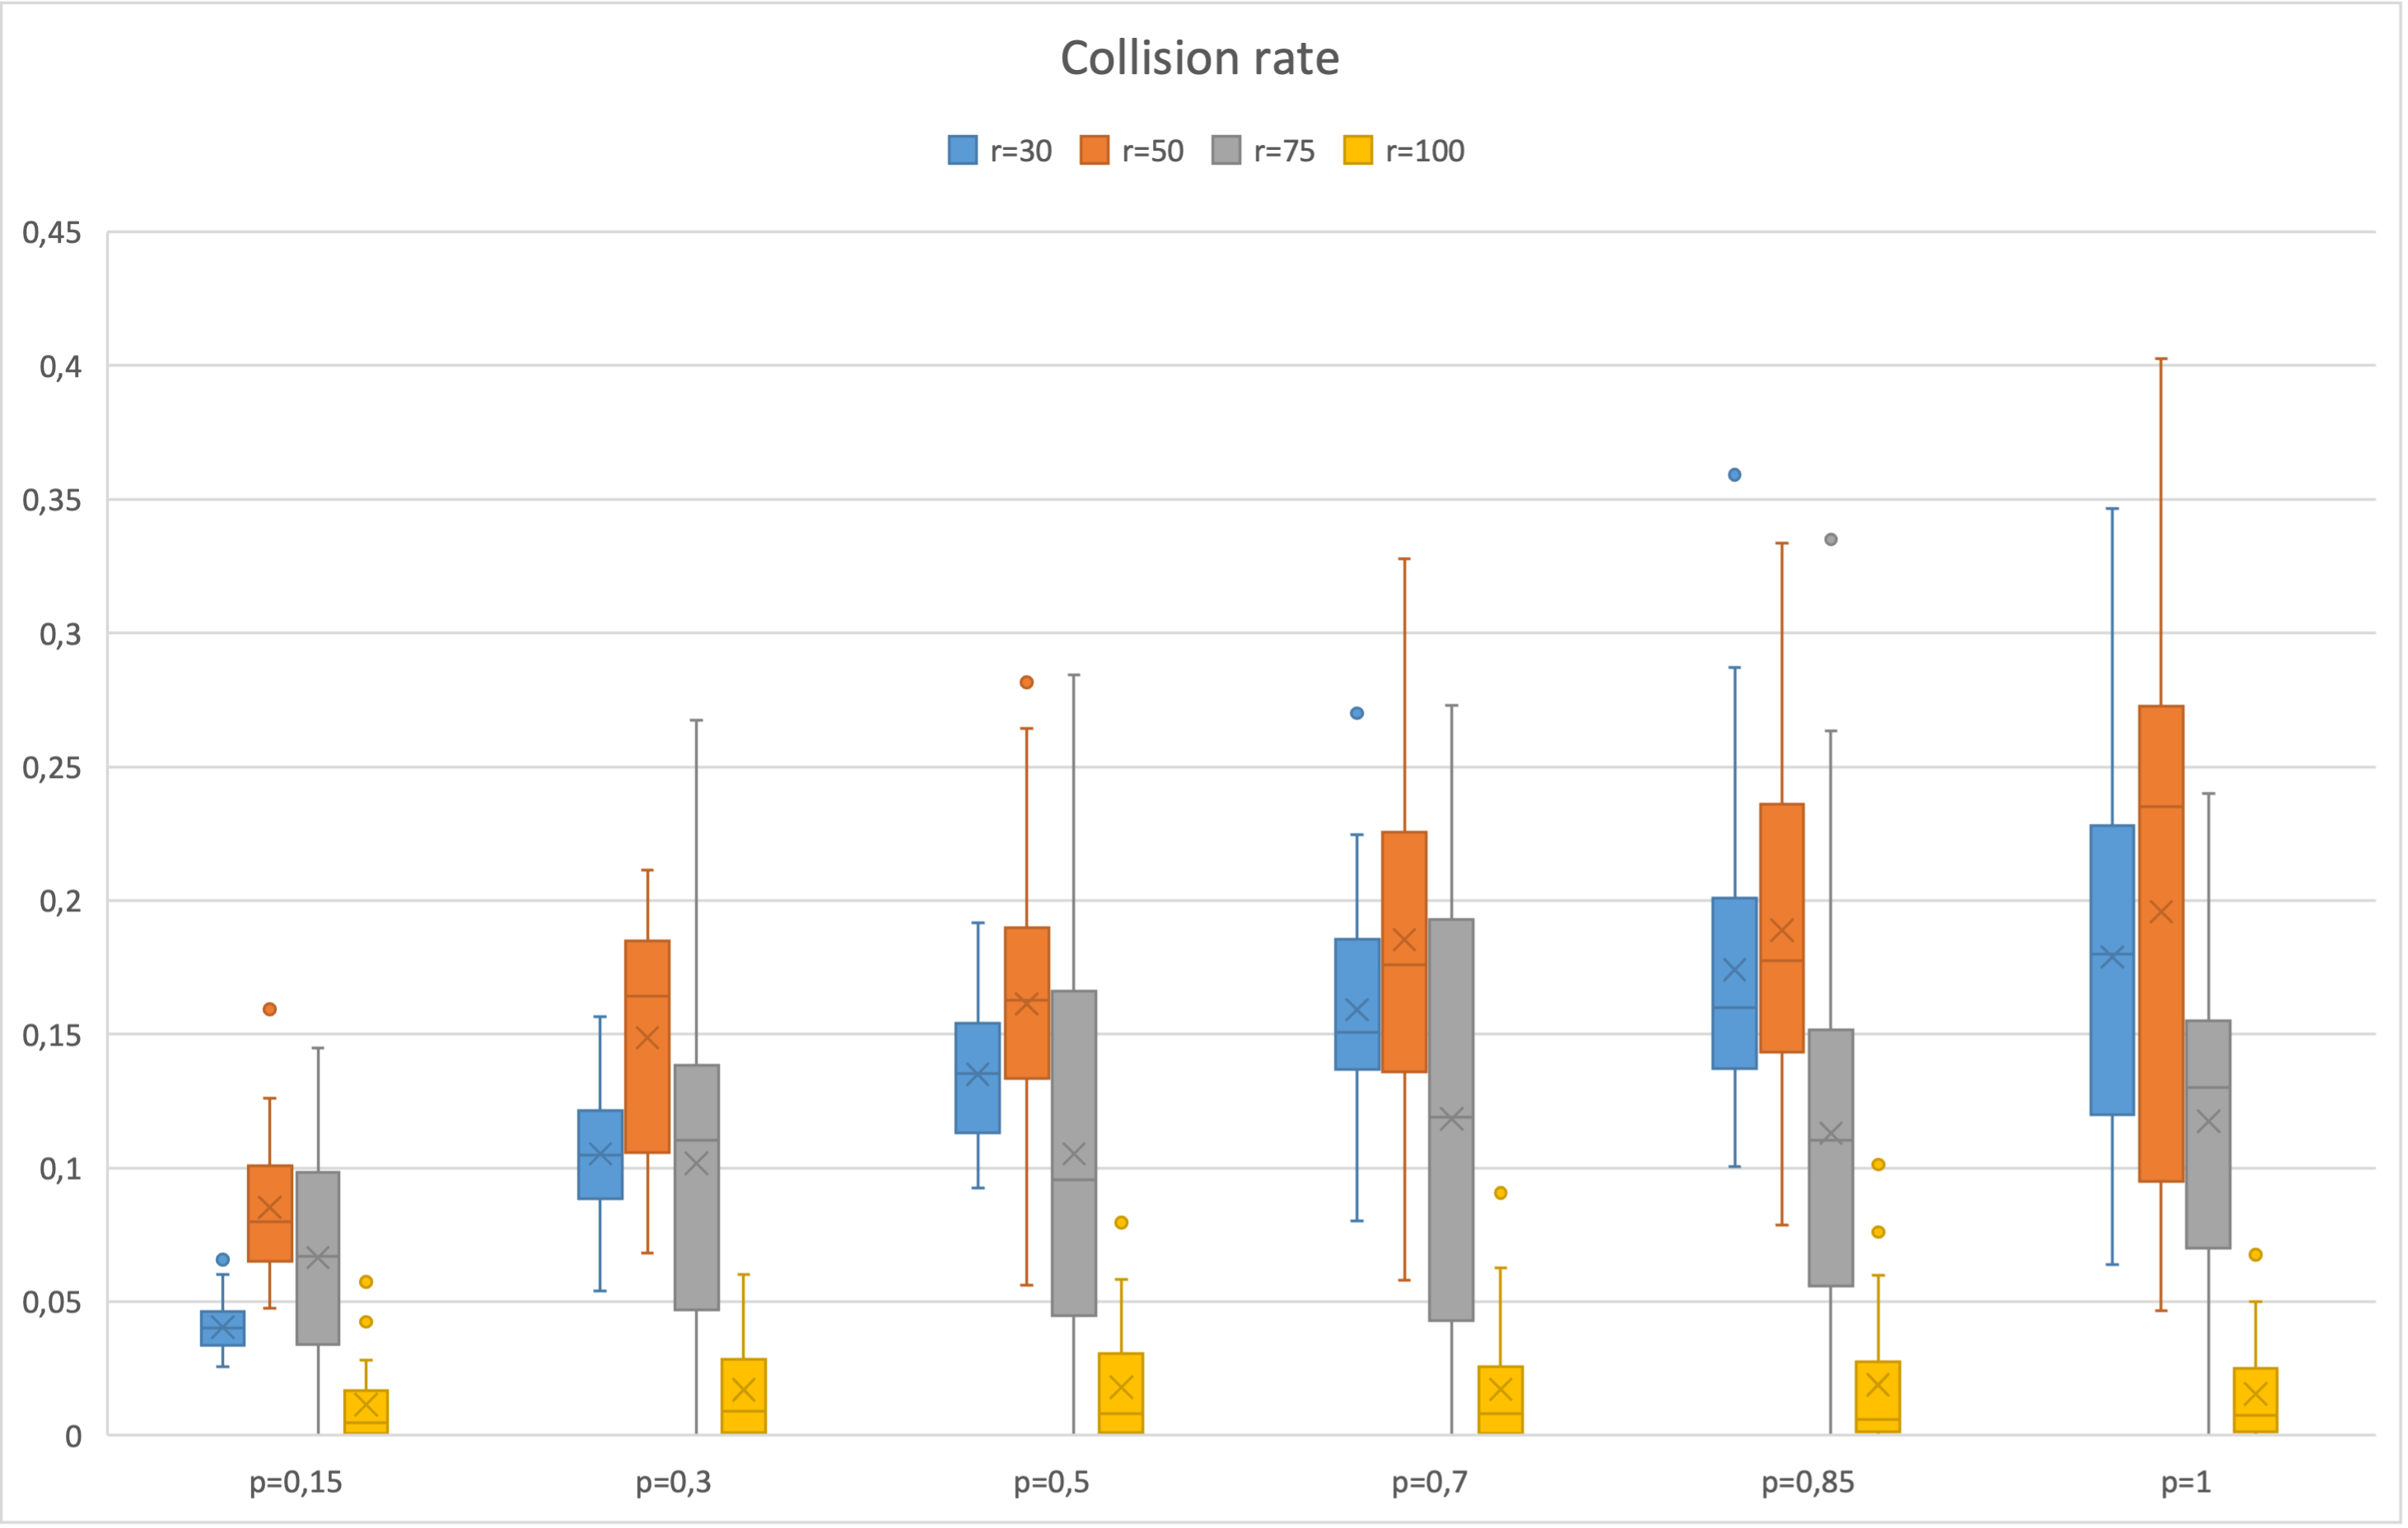
\includegraphics[width=\linewidth]{./images/Collision200Boxplot.png}
  \caption{200 Nodes}\label{fig:awesome_image2}
\endminipage
\end{figure}

\begin{figure}[H]
\minipage{0.50\linewidth}
  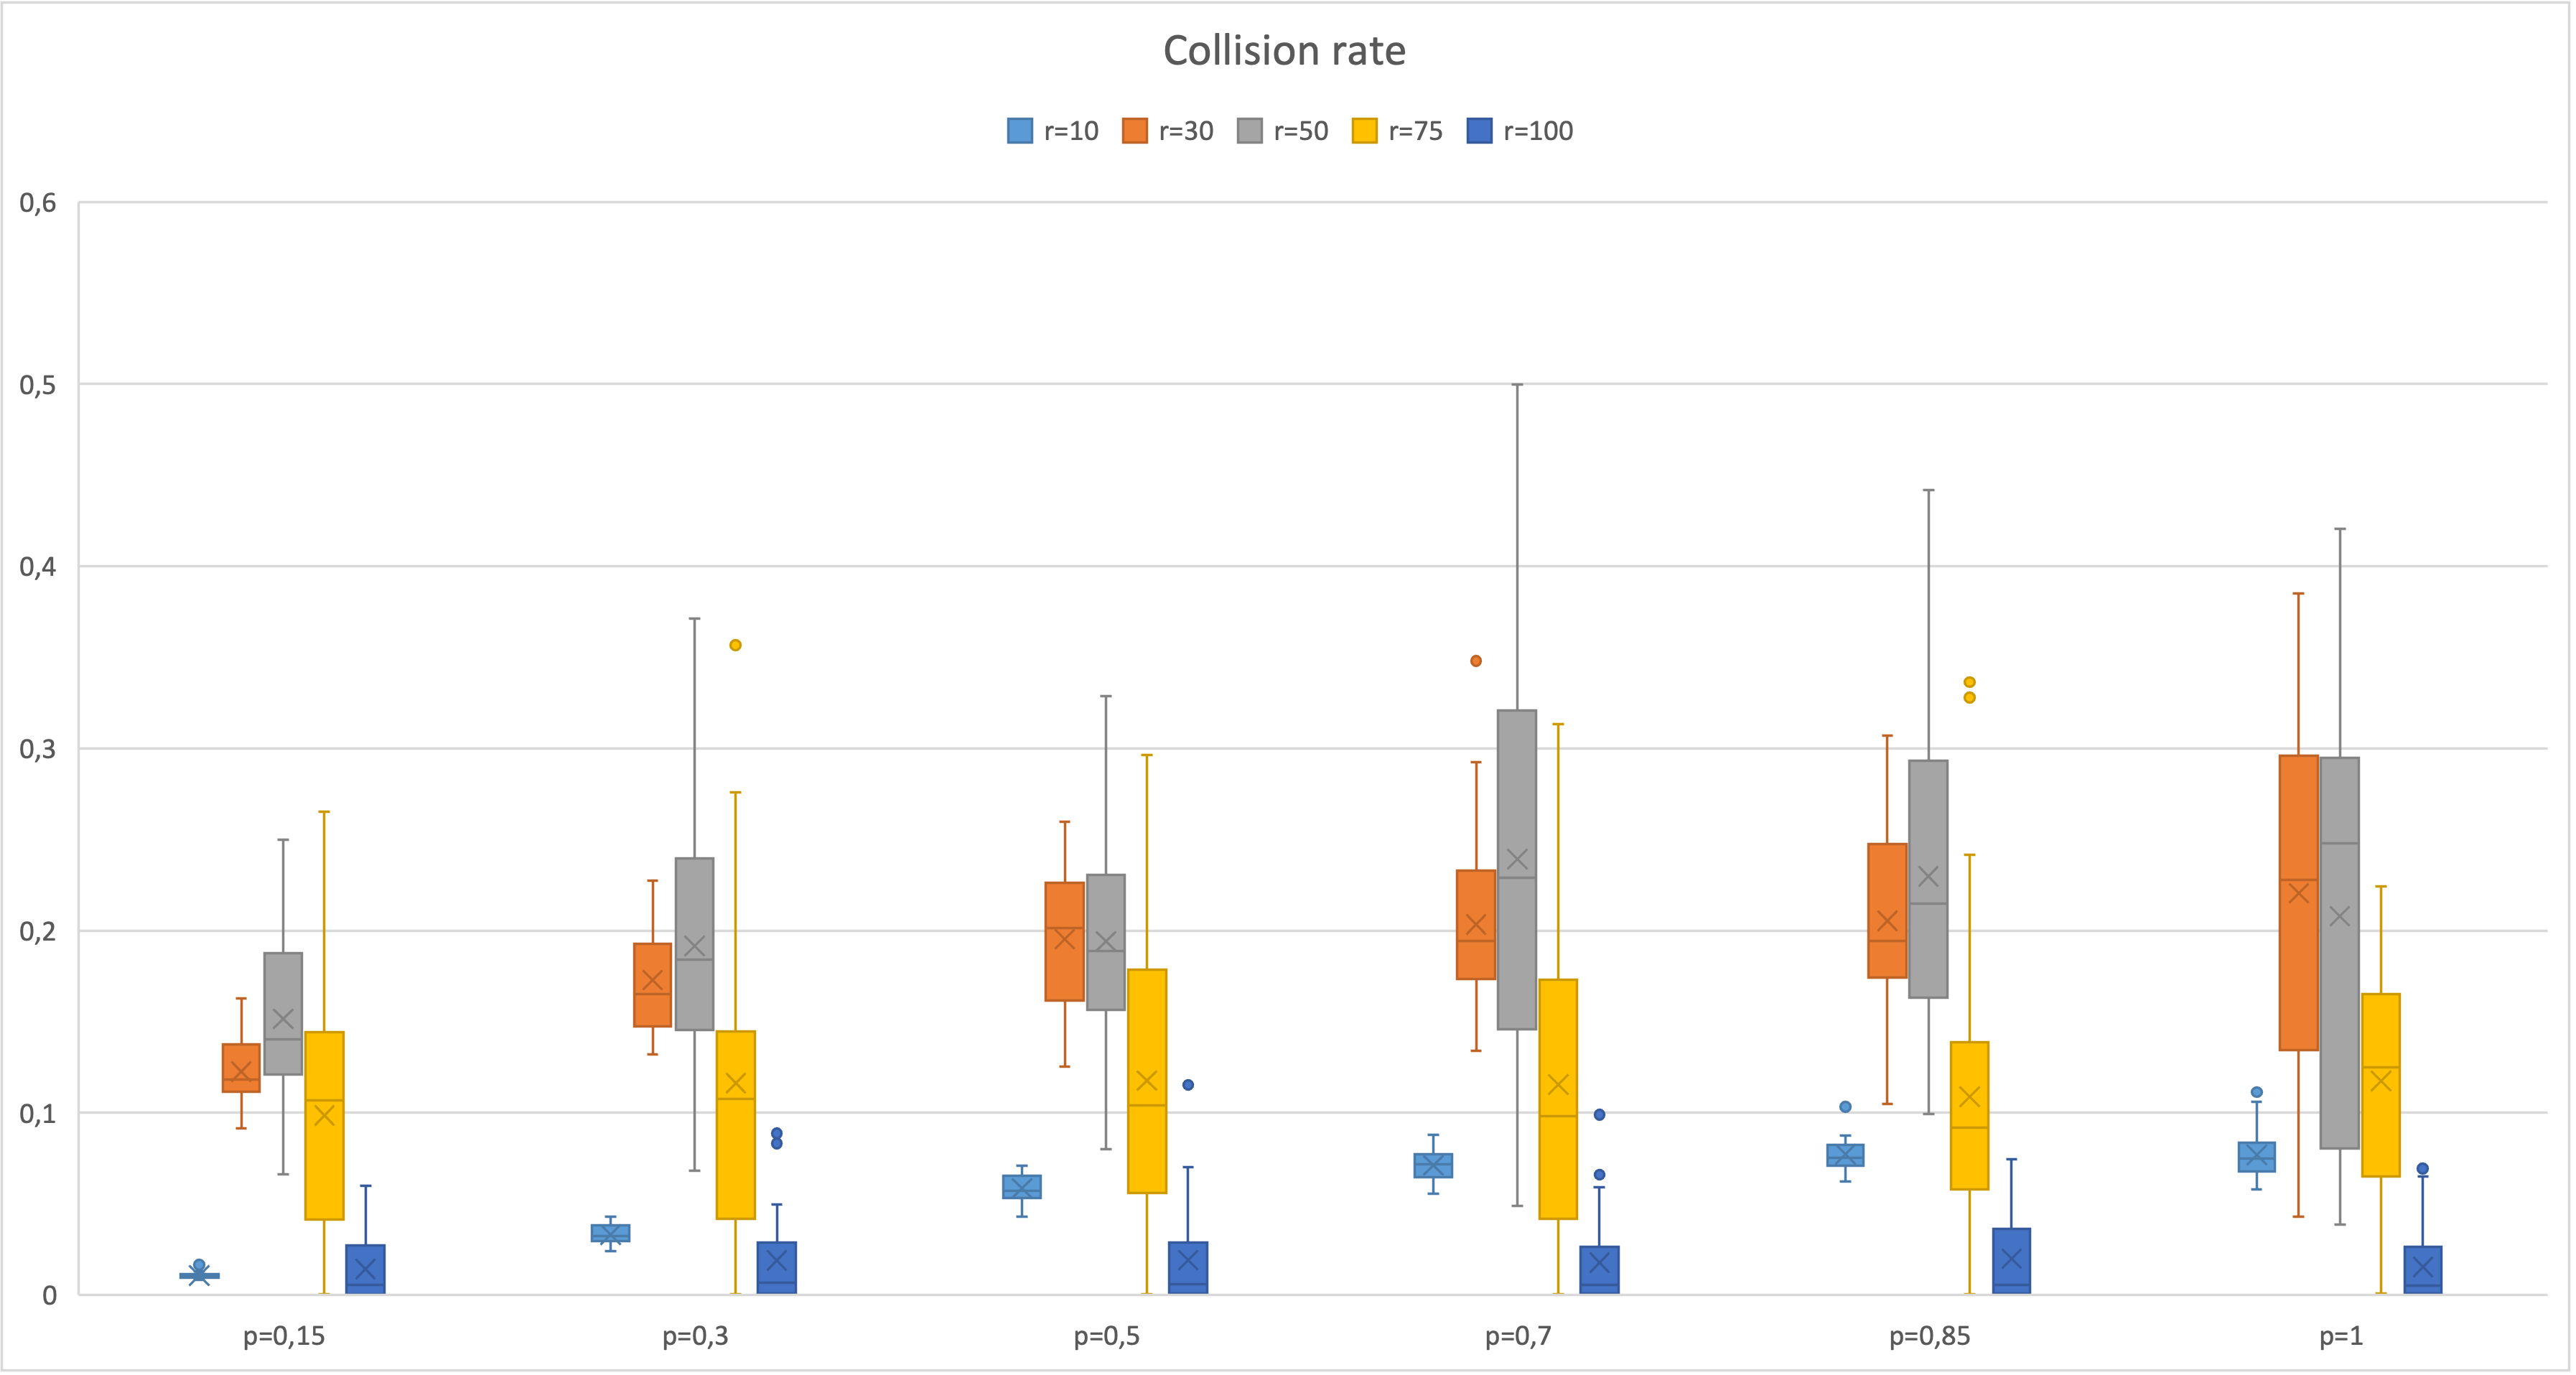
\includegraphics[width=\linewidth]{./images/Collision700Boxplot.png}
  \caption{700 Nodes}\label{fig:awesome_image1}
\endminipage\hfill
\minipage{0.50\linewidth}
  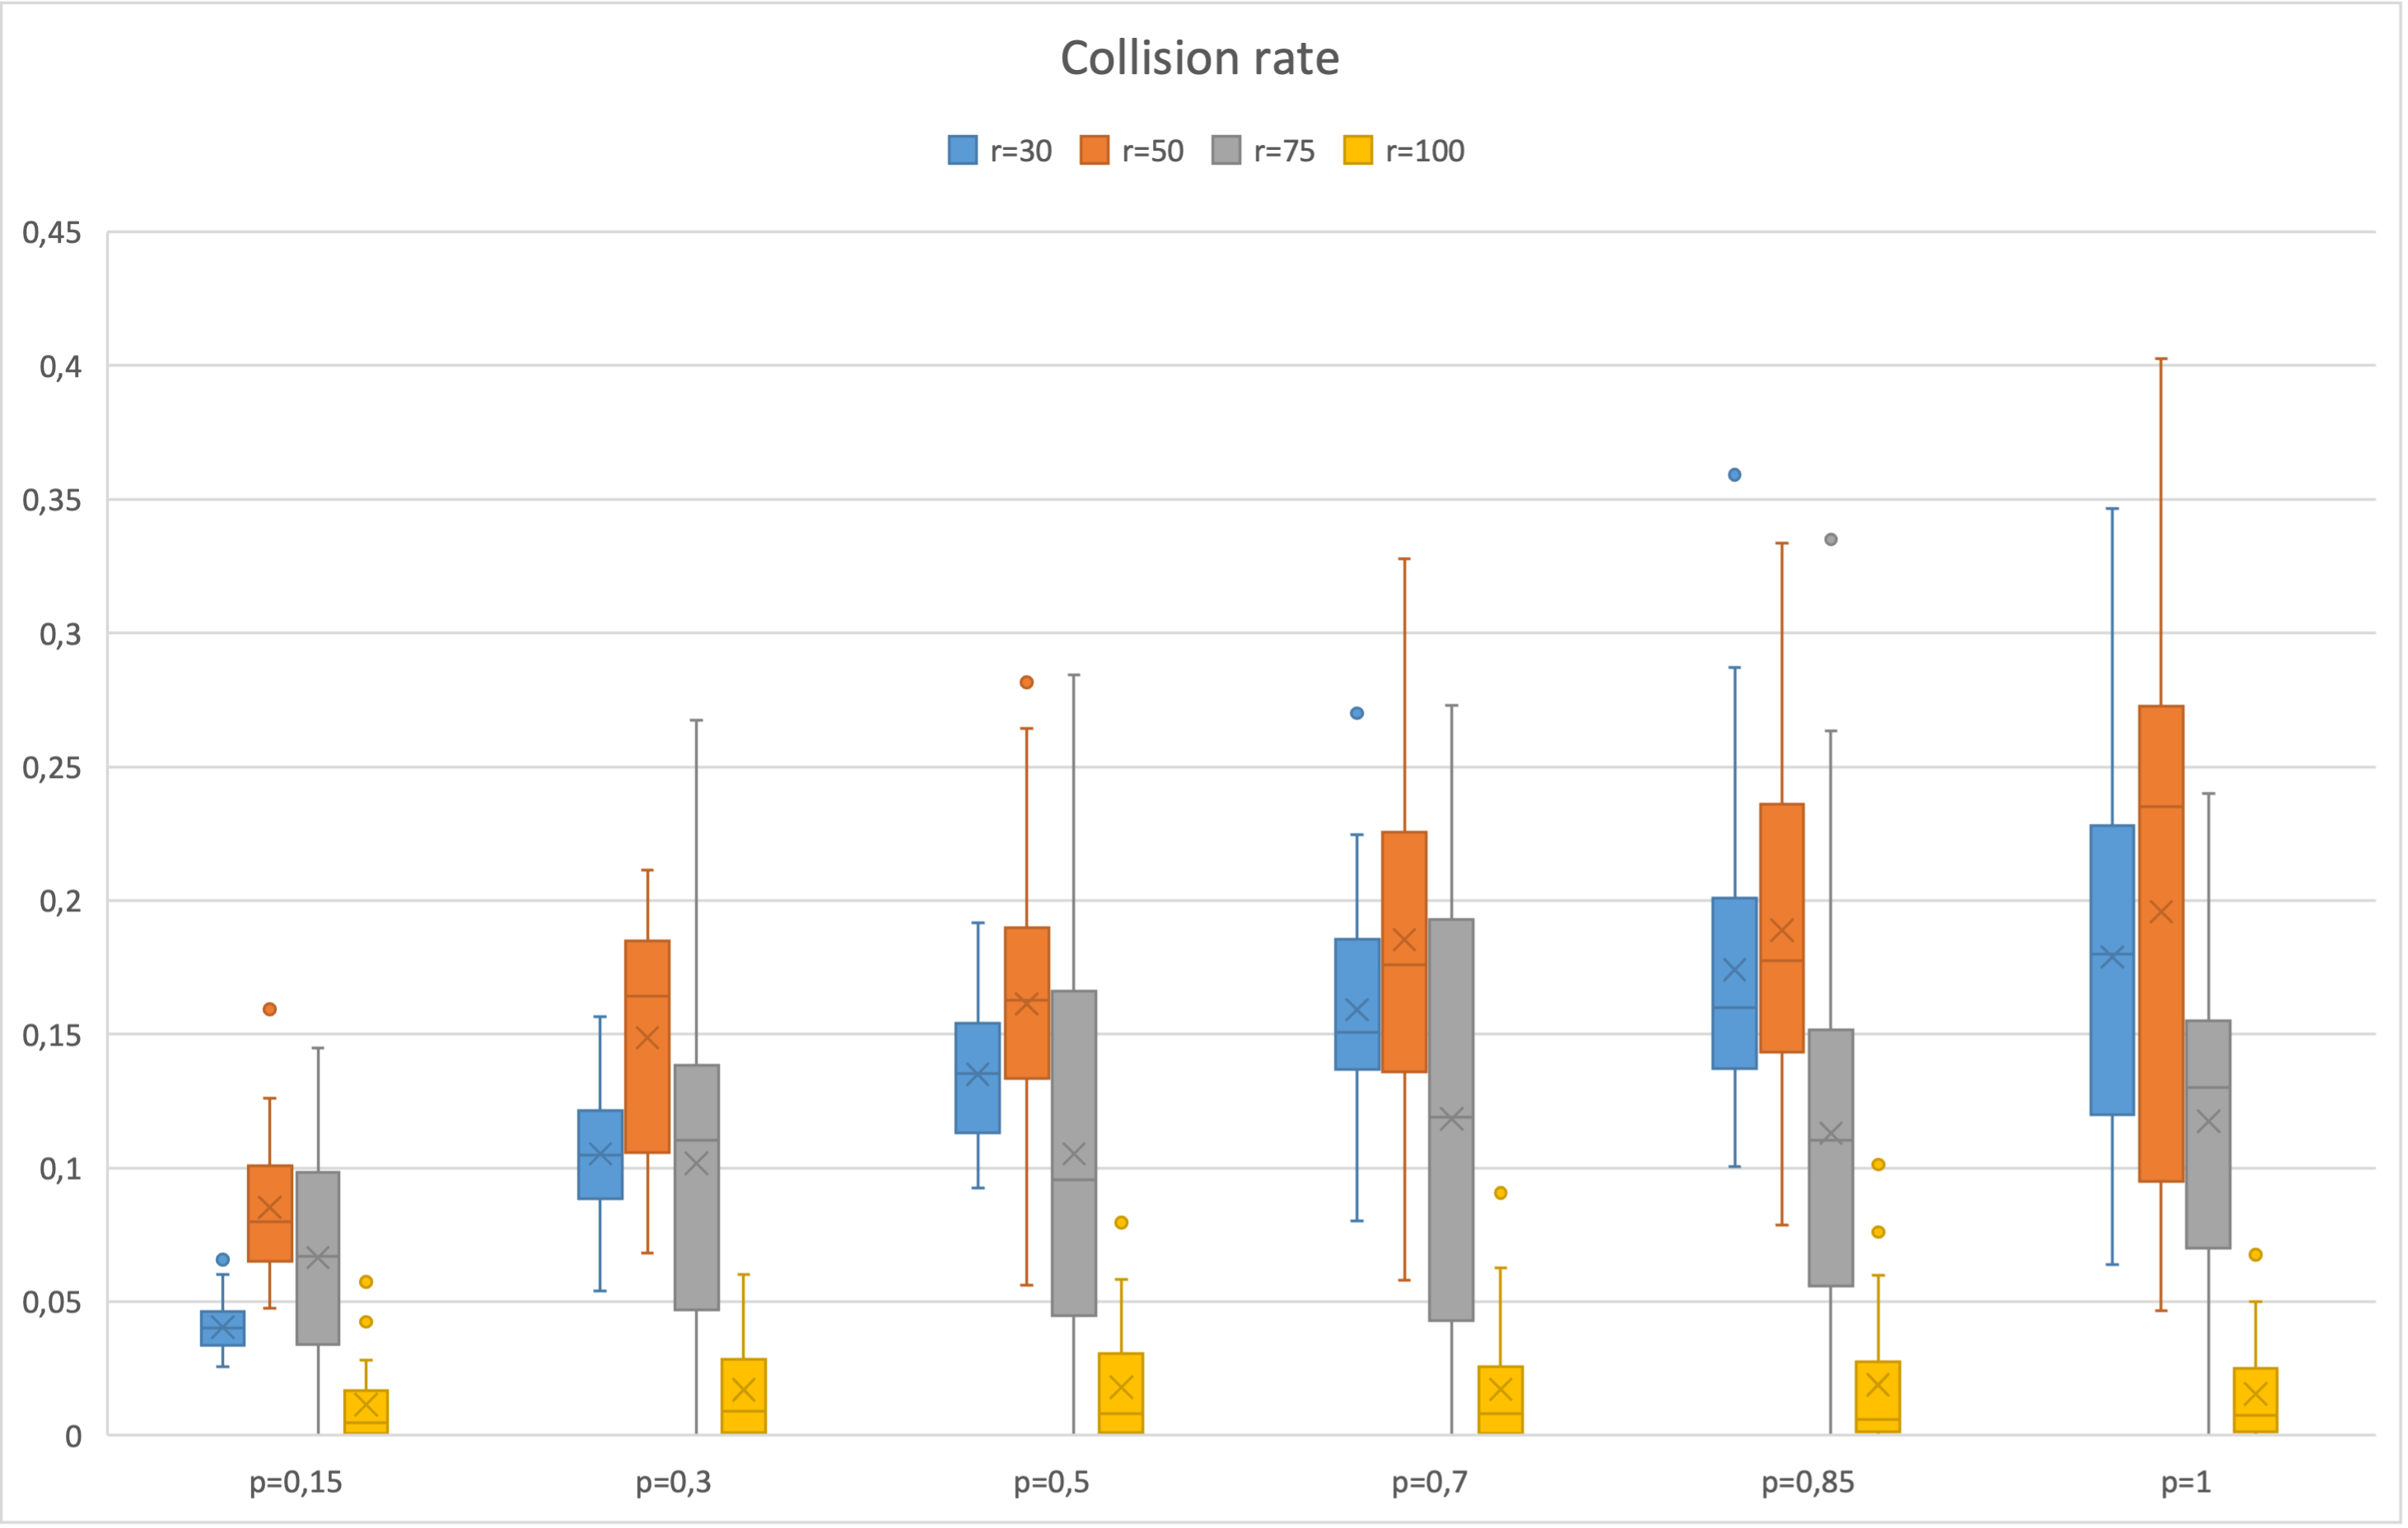
\includegraphics[width=\linewidth]{./images/Collision200Boxplot.png}
  \caption{200 Nodes}\label{fig:awesome_image2}
\endminipage
\end{figure}

By varying the number of nodes, the visible trends for the case of 200 nodes seem to be confirmed (insert quote). As regards the coverage time at low probabilities, an increase is noted, as expected, as the number of nodes increases.